% =====================================================================================================================
%  Long-range Ising Monte Carlo in d = 1, 2, 3: the thermal dimension Delta_epsilon(Delta_sigma).
%  Self-contained note (status 2026-10-13), released with the code and records in the MC/ folder of the public repository.
%  Compiles on its own with pdflatex (three passes); standard TeX Live packages only.
%  Every table body and plot coordinate is generated from the released records by code/package_tools/make_note_tables.py and pasted
%  verbatim; `make note-tables` regenerates them and checks that each generated line occurs in this file.
% =====================================================================================================================
\documentclass[10pt,a4paper]{article}
\usepackage[T1]{fontenc}
\usepackage[utf8]{inputenc}
\usepackage{lmodern}
\usepackage[margin=2.2cm]{geometry}
\usepackage{amsmath,amssymb}
\usepackage{booktabs,longtable,array}
\usepackage{rotating}
\usepackage{xcolor}
\usepackage{microtype}
\usepackage[shortlabels]{enumitem}
\usepackage{caption}
\usepackage{pgfplots}
\pgfplotsset{compat=1.16}
\usepackage{url}
\usepackage[hidelinks,pdftitle={Monte Carlo determination of the thermal dimension of the long-range Ising model in d=1,2,3},pdfauthor={Z. Zheng}]{hyperref}
\captionsetup{font=small,labelfont=bf}
\setlist{itemsep=1pt,topsep=3pt}
\emergencystretch=3em
\newcommand{\Ds}{\Delta_\sigma}
\newcommand{\De}{\Delta_\varepsilon}
\newcommand{\Deff}{\Delta_{\rm eff}}
\newcommand{\code}[1]{\texttt{#1}}
\newcommand{\lbl}[1]{{\mdseries\scshape #1}}
\newcommand{\sstat}{\sigma_{\rm stat}}
\newcommand{\ssys}{\sigma_{\rm sys}}
\newcommand{\ktau}{k_\tau}

\title{Monte Carlo determination of the thermal dimension $\De(\Ds)$\\ of the long-range Ising model in $d=1,2,3$\\[4pt]
\large Methods, data, results, limitations and reproduction}
\author{Z.~Zheng}  % author list as in the accompanying article
\date{Status of 15 October 2026}

\begin{document}
\maketitle

\begin{abstract}\noindent
We determine, by cluster Monte Carlo simulation, the scaling dimension $\De$ of the leading $\mathbb Z_2$-even scalar of the ferromagnetic
long-range Ising model with couplings $J(r)\propto r^{-(d+s)}$, as a function of the exactly known spin dimension $\Ds=(d-s)/2$, in $d=1,2,3$.
$\De$ is extracted from finite-size scaling of the scaled susceptibility and the Binder cumulants and their exact temperature derivatives.
The analysis rules were reviewed by a separate AI system (OpenAI Codex with the model gpt-6-astra, which also drafted the simulation
engines). In $d=2,3$ they were fixed before the production data were analyzed (one later
amendment is noted below); in $d=1$ they were revised after 8\,000 of the 10\,240 chains had been analyzed, and two gates were replaced after
couplings had failed them (section~\ref{sec:rules}). In $d=1$ ($N\le2^{19}$, 20 couplings) nine values pass the protocol, with statistical errors
$(2$--$5.5)\times10^{-4}$; they differ from the eight-loop resummed $\varepsilon$ expansion by $-0.0024$ to $+0.0032$, up to 13 times their
statistical errors. Their systematic error is the half-range of a family of fit models, a sensitivity scale rather than a standard deviation,
and an audit by the same AI system finds the values at three couplings sensitive to the size cut or the correction model. At the three
couplings closest to the Gaussian end ($\varepsilon\le0.15$) the Monte Carlo values lie $0.0065$--$0.0104$ below the expansion. In $d=2$
($L\le1024$) the finite-size effective dimensions are precise ($\sigma\approx0.002$) and agree with the resummed expansion to $0.0015$ for
$s=1.2$--$1.4$, about as well as the expansion itself is determined there; no infinite-size value passes the protocol. In $d=3$ ($L\le128$) one
value passes, $\De(s{=}1.6)=1.47314\pm0.00118\,(\mathrm{stat})\pm0.00230\,(\mathrm{sys})$, only under an amendment adopted after the data had been
evaluated; it agrees with the expansion ($1.4721$). Near the short-range end the 3D extrapolations lie $0.022$--$0.033$ above the expansion.
We describe the model, algorithms, data, rules, results and limitations, and how to reproduce every number from the released records.
\end{abstract}

\tableofcontents
\clearpage

% =====================================================================================================================
\section{Overview}\label{sec:overview}
\subsection{Scope}
This note is written for a physicist outside the project. It explains the problem and what is known exactly (section~\ref{sec:model}), the
Monte Carlo and analysis methods in enough detail to re-implement them (sections~\ref{sec:mc}--\ref{sec:labels}), how and when the analysis
rules were fixed (section~\ref{sec:rules}), all results including negative ones (sections~\ref{sec:1d}--\ref{sec:3d}), the limitations and
open problems (sections~\ref{sec:synthesis}--\ref{sec:open}), and how to recompute every number from the released code and records
(section~\ref{sec:repro}). The work was carried out by AI agents under the direction of the author. The simulation engines (section~\ref{sec:mc}) were
drafted by GPT-6 astra (OpenAI, via ChatGPT) in discussions with the author and supplied as three separate packages: the initial 1D package (reference engine, campaign tools
and analysis core), the specialized 1D engine, and the 2D/3D engine. The fit pipelines, protocols, evaluators and analyses were written by
Claude (Anthropic) agents. Protocols and code were reviewed by a second AI system, OpenAI Codex with the model gpt-6-astra, the same model that
drafted the engines, in sessions separate from the ones that wrote the protocols and fits. There was no human referee. Numbers in tables and figures are generated by script from
the production records; nothing here is a new measurement except the diagnostics explicitly marked as such.

\subsection{Headline results}
\begin{table}[htbp]\centering\small
\caption{What the Monte Carlo establishes. ``Passes the protocol'' means the label \lbl{accepted} or \lbl{accepted ($\ssys$-dominated)} of
section~\ref{sec:labels}; it is a statement about the protocol (in $d=3$ as amended by P1, section~\ref{sec:p1}), not a guarantee of
correctness. The theory comparison uses the eight-loop resummed $\varepsilon$ expansion of the accompanying article~\cite{Zheng:2026ai}
(CB8, section~\ref{sec:theory1d}).}\label{tab:headline}
\begin{tabular}{@{}>{\raggedright\arraybackslash}p{0.7cm}>{\raggedright\arraybackslash}p{7.2cm}>{\raggedright\arraybackslash}p{7.6cm}@{}}\toprule
$d$ & result & limitations \\\midrule
1 & Nine of 20 couplings pass the protocol: $\De$ with $\sstat=(2.0$--$5.5)\times10^{-4}$ and $\ssys=(0.8$--$9.6)\times10^{-3}$ (table~\ref{tab:1dfinal}); they differ from the resummed $\varepsilon$ expansion by $-0.0024$ to $+0.0032$ (table~\ref{tab:theory1d}). &
$\ssys$ is a model-family half-range; the values at $\Ds=0.025$, $0.175$, $0.225$ are sensitive to the size cut or correction model; two labels ($0.1625$, $0.1727335$) depend on the platform; quoted fits at $0.1$ and $0.125$ have $P_{\chi^2}\approx5\times10^{-5}$; for $\Ds\ge0.0875$ the fit lies above the crossing extrapolation by a common $+0.0010(3)$ (section~\ref{sec:robust}). At $\Ds=0.2125$--$0.2375$ the Monte Carlo values are $0.0065$--$0.0104$ below the expansion. \\
2 & Finite-size effective dimensions $\Deff(U_4,512\to1024)=0.958$--$0.977$ with $\sigma\approx0.002$ at all eight couplings; they agree with the resummed expansion to $0.0015$ for $s=1.2$--$1.4$, where the expansion itself depends on how its end point is imposed by up to $0.005$ (table~\ref{tab:theory23}). &
No infinite-size value passes the protocol. Two single-series extrapolations ($s=1.05,1.1$) lie $0.05$--$0.065$ below the expansion; near both ends of the window the finite-size values drift away from it. \\
3 & One value passes, $\De(s{=}1.6)=1.47314\pm0.00118\pm0.00230$, consistent with the expansion ($1.4721$) and with the finite-size $\Deff(U_4,64\to128)=1.4715(31)$. &
Accepted only under amendment P1, adopted after the data were evaluated, whose last code fixes are uninspected. Near the short-range end the extrapolations are $0.022$--$0.033$ above the expansion, and the $Y$ and $U_4$ estimates split. \\\bottomrule
\end{tabular}
\end{table}

% =====================================================================================================================
\section{The model and what is known exactly}\label{sec:model}
\subsection{Hamiltonian and conventions}
Ising spins $S_i=\pm1$ on a periodic hypercubic lattice of linear size $L$ ($N=L^d$ sites) interact through the fully periodized power law
\begin{equation}
 H=-\sum_{i<j}J_L(i-j)\,S_iS_j,\qquad J_L(\mathbf r)=\sum_{\mathbf n\in\mathbb Z^d}|\mathbf r+L\mathbf n|^{-d-s}\quad(\mathbf r\not\equiv0\bmod L),
 \label{eq:H}
\end{equation}
with no Kac normalization (the nearest-neighbor coupling of the infinite lattice is one) and no extra short-range term. Inverse temperatures
$\beta$, including critical ones, are quoted in this normalization. Below, a \emph{coupling} always means one value of $s$ (equivalently of
$\Ds$) on the simulation grid. In $d=1$ the lattice size is denoted $N$, and
$J_N(r)=N^{-1-s}[\zeta(1+s,r/N)+\zeta(1+s,1-r/N)]$ with the Hurwitz zeta function.

\subsection{Long-range fixed points and their correction exponents}
For $d/2<s<s_*$ the critical point is the long-range fixed point~\cite{Fisher:1972zz,Sak:1973oqx,Paulos:2015jfa}. Because the kinetic term is
non-local, the spin field is not renormalized and
\begin{equation}
 \Ds=\frac{d-s}{2}\qquad\text{exactly},
\end{equation}
i.e.\ $\eta=2-s$. The thermal dimension $\De$ (dimension of the leading $\mathbb Z_2$-even scalar, $1/\nu=d-\De$) is the unknown. The ends of the
window and the leading corrections to scaling are:
\begin{itemize}
\item \emph{Gaussian end} $s\to d/2$: mean field, $\De\to d-s=d/2$. With $\varepsilon=2s-d$, $\De=d-s+\varepsilon/3+O(\varepsilon^2)$; the
 $\phi^4$ coupling is nearly marginal and the leading correction exponent is $\omega=\varepsilon+O(\varepsilon^2)$, so corrections are slow
 ($\omega\approx\varepsilon$, which is 0.05 at the $d=1$ coupling closest to this end and 0.1 in $d=2,3$).
\item \emph{Short-range end} $s\to s_*=2-\eta_{\rm SR}$ ($d=2,3$; Sak's criterion~\cite{Sak:1973oqx}): $s_*=7/4$ in $d=2$, $s_*\simeq1.963702$
 in $d=3$, where $\De\to\De^{\rm SR}=1$ ($d=2$) and $1.412625$ ($d=3$; the 3D values from the conformal bootstrap~\cite{Chang:2024whx}). Near $s_*$ the fixed point is the short-range Ising fixed point
 weakly coupled to a generalized free field $\chi$ through $g\int\sigma\chi$~\cite{Behan:2017dwr,Behan:2017emf}: with $\delta=(s_*-s)/2$,
 $dg/d\ell=\delta g-\beta_3g^3$, where $\ell$ is the logarithm of the length scale, and $\gamma_\varepsilon\equiv\De-\De^{\rm SR}=c_\varepsilon
 g^2$, with $\beta_3=12.26(3)$ and $c_\varepsilon=3.3(5)$ in $d=3$~\cite[eqs.~(2.24), (3.41)]{Behan:2017emf} (and $\gamma_\varepsilon=O(\delta^2)$ in
 $d=2$). The $\sigma\chi$ coupling approaches its fixed point as $\ell^{-(s_*-s)}$, a slow correction with
 exponent $s_*-s=2\delta$ ($0.05$ at 2D $s=1.7$, $0.014$ at 3D $s=1.95$). A lattice model with a pure power law starts at strong bare
 coupling, so the approach is a crossover rather than a small correction. It may contribute to the $Y$--$U_4$ splits seen near $s_*$, but in
 $d=3$ the split grows with $L$, whereas at leading order this flow makes it shrink (sections~\ref{sec:2d}, \ref{sec:3d}).
\item \emph{$d=1$, $s\to1$} ($\Ds\to0$): the chain approaches the inverse-square point~\cite{Kosterlitz:1976zz,Cardy:1981xx}, where the
 thermal perturbation becomes marginal ($\De\to1$); the leading correction exponent tends to zero together with the thermal exponent
 $y_t=1-\De$ (at leading order of the Kosterlitz flow they are equal). Our fits near this end indeed give $\omega\approx y_t$ (table~\ref{tab:robust}).
\end{itemize}
In $d=2$ both ends have $\De=1$, so $\De(s)$ dips below 1 in the interior; in $d=3$ it interpolates between $1.5$ and $1.4126$.

\subsection{Observables and the effective dimension}
With $m=N^{-1}\sum_iS_i$ define the scaled second moment, the Binder cumulant~\cite{Binder:1981sa} and higher moment ratios
\begin{equation}
 Y=L^{2\Ds}\langle m^2\rangle,\quad U_4=1-\frac{\langle m^4\rangle}{3\langle m^2\rangle^2},\quad
 U_6=\frac{\langle m^6\rangle}{15\langle m^2\rangle^3},\quad U_8=\frac{\langle m^8\rangle}{105\langle m^2\rangle^4}.
\end{equation}
All are dimensionless at criticality up to corrections and are functions of the scaling variable $(\beta-\beta_c)L^{d-\De}$. For a
size-doubling pair $(L,2L)$ let $\beta_\times$ be the crossing $U_4^{(L)}(\beta_\times)=U_4^{(2L)}(\beta_\times)$. At this same temperature
\begin{equation}
 \Deff^{Q}(L)=d-\log_2\frac{Q'_{2L}(\beta_\times)}{Q'_L(\beta_\times)},\qquad Q\in\{U_4,U_6,U_8,Y\},\quad Q'=\partial_\beta Q
 \label{eq:Deff}
\end{equation}
(the quotient method~\cite{Ballesteros:1996bd}). Every $Q$ gives $\De$ as $L\to\infty$; their differences at finite $L$ measure corrections to
scaling. In $d=1$ the Binder cumulant is written $U$ and sizes are $N$.

% =====================================================================================================================
\section{Monte Carlo method}\label{sec:mc}
\subsection{Cluster algorithm}
All simulations use the extended-Poisson Swendsen--Wang~\cite{Swendsen:1987ce} construction of Fukui and Todo~\cite{Fukui:2009on}, whose cost
per sweep is $O(N)$ for long-range couplings (see also ref.~\cite{Luijten:1995mc}; for an application to the long-range Ising model,
ref.~\cite{Horita:2017ul}). Per sweep a Poisson number of candidate bond events is
drawn with mean $\beta N\sum_{\mathbf r}J(\mathbf r)$; each event picks a uniform source site and a displacement $\mathbf r$ with probability
$\propto J(\mathbf r)$, so each unordered pair receives events at rate $2\beta J_{ij}$. An event is kept only if the two spins are aligned;
kept bonds are joined by union--find and every cluster receives an independent random sign. The number of kept events, $K$ (counted with
multiplicity, including repeated and cycle-closing events), makes the weight of a bond configuration proportional to $\beta^K$; cumulants of
$K$ therefore give exact $\beta$-derivatives and exact multi-temperature reweighting.

\subsection{Engines}
\begin{description}[leftmargin=1.2em]
\item[$d=1$, reference engine] (\path{code/1d/src/lri_mc.cpp}, C++17): Walker alias table over all $N-1$ displacements, Mersenne twister,
 checkpoint/restart with atomic writes, one completion record per chain. Used for the pilot, the two-point campaign and stages 0, A and B (the $d=1$ campaigns of table~\ref{tab:campaigns}).
\item[$d=1$, specialized engine] (\path{code/1d/src_1d/}): alias table for $r<256$, geometric envelope with rejection for the tail,
 xoshiro256++ generator; 1.5--2.1$\times$ faster single core and 2.5--3.3$\times$ faster when 30 chains share a node. It agrees with the
 reference engine within statistics on 24 observable comparisons. Used for the N2 campaign (table~\ref{tab:campaigns}).
\item[$d=2,3$] (\path{code/2d3d_engine/code/src/}): exact periodic-image sampling without an $L^d$ coupling table. Displacements in the core
 cube $[-16,15]^d$ use exact weights via an alias table; the rest is a union of shells $C_{k+1}\setminus C_k$, $C_k=[-16\cdot2^k,16\cdot2^k-1]^d$,
 sampled from the envelope $(16\cdot2^k)^{-d-s}$ with rejection and folded modulo $L$; the 8 (2D) or 26 (3D) nearest offsets are separate
 Poisson processes. Records per sweep: $K$, improved estimators of $m^2,m^4,m^6,m^8$ from the cluster fractions $c_j$
 ($S_{2k}=\sum_jc_j^{2k}$: $m_2=S_2$, $m_4=3S_2^2-2S_4$, $m_6=15S_2^3-30S_2S_4+16S_6$,
 $m_8=105S_2^4-420S_2^2S_4+140S_4^2+448S_2S_6-272S_8$), the sampled $m^2$, the largest cluster and the number of clusters. The engine was
 checked against exact enumeration of $4\times4$ and $2^3$ systems and against the reference engine, and restarts reproduce bitwise.
\end{description}

\subsection{Derivatives and reweighting}
For a graph observable $A$, $\partial_\beta\langle A\rangle=\mathrm{Cov}(A,K)/\beta$ and
$\partial_\beta^2\langle A\rangle=[\langle A(K-\bar K)^2\rangle-\langle A\rangle\mathrm{Var}K-\mathrm{Cov}(A,K)]/\beta^2$ (the last term arises
because the weight is $\beta^K$). In $d=1$ the analysis keeps, per $(N,\beta)$, the six quantities $(Y,Y',Y'',U,U',U'')$ with a $6\times6$
jackknife covariance from blocks of 2048, 4096 (primary) and 8192 sweeps. In $d=2,3$ each chain is packed into histograms in $K$ at blocks of
1000, 2000 (primary) and 4000 sweeps, and the five simulated temperatures of a size are combined by multi-temperature reweighting
(MBAR~\cite{Shirts:2008xx}, the multiple-histogram method~\cite{Ferrenberg:1989ui}) with the exact factor $(\beta/\beta_0)^K$.

\subsection{\texorpdfstring{Crossings and bootstrap in $d=2,3$}{Crossings and bootstrap in d=2,3}}
For each pre-registered pair, the crossing $\beta_\times$ is the unique root of $U_4^{(2L)}-U_4^{(L)}$ inside the shared temperature bracket
(exactly one root required, reweighting effective sample size $\ge0.2$). Errors come from 500 joint bootstrap draws (seed 571239): in each draw the blocks of every chain are resampled once (multinomial
weights), the same resample serves both pairs that contain that size, and crossings and slopes are recomputed; the draws give the full covariance across pairs and
observables.

\subsection{Equilibration and provenance}
Every $(L,\beta)$ group has hot and cold replicas with $5\times10^4$ warm-up sweeps. In $d=2,3$ the equilibration rule of a coupling requires
(i) every chain's block mean of $m^2$ within $|z|\le4$ of its group, and at most 2\,\% of the coupling's chains beyond $|z|=3$; and (ii) no
group in which half or more of the chains fail the drift test (first against second half of the chain, $|z|\le4$), the condition block
length $\ge20\,\tau_{\rm int}$ at every block size used, or finiteness. In $d=3$ the rule is also applied to the reblocking records. In $d=1$
(protocol v3) every group must have its hot--cold difference and every replica's first--second-half difference within $|z|\le4$ and
$\tau_{\rm int}$ below block$/20$; across the coupling at most 2\,\% of the groups may exceed $|z|=3$ in the hot--cold test and at most 2\,\% of
the replicas in the half-chain test. A failure labels the coupling \lbl{equilibration failed}; no chain is removed. In the preflight runs
(short runs at the production sizes, before each production, that check rates, autocorrelation times and crossing brackets) $\tau_{\rm int}$
was at most 17 sweeps ($d=1$), 29 ($d=2$, $L=1024$) and 34 ($d=3$, $L=128$). Each chain writes a
completion record; snapshot manifests list the SHA-256 of every summary, block archive, registry and code file; output directories are
created afresh and never overwritten.

% =====================================================================================================================
\section{How a label is assigned}\label{sec:labels}
Each coupling receives exactly one label from a fixed decision table, applied in the order of table~\ref{tab:labels}; the first condition that
applies gives the label. Only the two \lbl{accepted} labels denote values that passed the protocol (in $d=2,3$ the frozen rule or, where it
is calibrated, amendment P1; section~\ref{sec:p1}). A \emph{gate} is a pass/fail condition on a fit or an extrapolation series; a $d=1$ fit that
passes its gates is \emph{quotable} (section~\ref{sec:v3}), and a $d=2,3$ series that passes its gates is \emph{eligible}
(section~\ref{sec:proto23}).

\paragraph{The two errors.} $\sstat$ is a bootstrap error of the quoted value. $\ssys$ is half the range of the quoted values over a family of
admissible fit models (in $d=1$) or extrapolation series (in $d=2,3$): a \emph{model-family sensitivity scale}, not a standard deviation and
not a bound. It covers only the variation inside that family, it is symmetric about the quoted value although the family's excursions need not
be, and there is no justified rule for adding it to $\sstat$ in quadrature. Values are written $v(\sstat)(\ssys)$ in units of the last digits.

\begin{table}[htbp]\centering\small
\caption{The decision labels and what triggers them. ``Cross-check'': two extrapolations of the same data (in $d=1$ the global fit and the
crossing series, in $d=2,3$ the $U_4$ and $Y$ series) must agree within $2\sigma_D$, $\sigma_D$ being the error of their paired
difference.}\label{tab:labels}
\begin{tabular}{@{}>{\raggedright\arraybackslash}p{3.2cm}>{\raggedright\arraybackslash}p{6.1cm}>{\raggedright\arraybackslash}p{6.1cm}@{}}\toprule
label & trigger in $d=1$ & trigger in $d=2,3$ \\\midrule
\lbl{equilibration failed} & a group fails the equilibration rule & same \\
\lbl{coverage-limited} & a pre-registered size or temperature missing & a pre-registered pair missing \\
\lbl{model-limited} & no fit passes the quality gates (finite-size values reported) & no extrapolation series is eligible \\
\lbl{conditional} & a quoted fit exists but $\ssys$ is not available: fewer than four quotable fits, or fewer than two minimum sizes or two variants among them & exactly one eligible series, so no $\ssys$ \\
\lbl{reblocking failed/unavailable} & $\sstat$ at blocks 2048 or 8192 outside $\pm30\,\%$ of the primary & same at blocks 1000 or 4000 \\
\lbl{cross-check unavailable} & fewer than two eligible crossing series & $U_4$ and $Y$ not both eligible \\
\lbl{cross-check failed} & global fit and median crossing extrapolation differ by more than $2\sigma_D$ & extrapolated $U_4$ and $Y$ differ by more than $2\sigma_D$ \\
\lbl{accepted} & none of the above & none of the above \\
\lbl{accepted ($\ssys$-dominated)} & accepted and $\ssys>3\times$ the median $\sstat$ of the quotable fits & -- \\\bottomrule
\end{tabular}
\end{table}
Suffix ``[$\sigma$]'' ($d=2,3$): $\sigma(\Deff^{U_4})$ of the largest pair exceeds the target 0.003. A label is prefixed \lbl{non-production}
when the provenance checks of its inputs do not pass. Tables abbreviate cross-check to x-check, unavailable to unavail., dominated to dom.,
reblocking to reblock.\ and equilibration to equil.

% =====================================================================================================================
\section{How the rules were fixed}\label{sec:rules}
The aim was to write each analysis protocol, and have it reviewed, before the data it governs were analyzed, with selection rules blind to
$\De$. Table~\ref{tab:timeline} records how far this held. Reviews were done by the second AI system named in section~\ref{sec:overview}:
plan reviews of the protocol texts, each ending with the verdict ``approved'' (no unresolved material defect in the reviewed revision) or
``revise'', and inspections of the code that implements them. The protocol texts, their hashes and their review status
are released with the code (appendix~\ref{app:hashes}); \code{REVIEWS.md} summarizes every review round and verdict.
\begin{table}[htbp]\centering\small
\caption{When the rules were fixed, relative to the data they govern.}\label{tab:timeline}
\begin{tabular}{@{}>{\raggedright\arraybackslash}p{2.9cm}>{\raggedright\arraybackslash}p{5.6cm}>{\raggedright\arraybackslash}p{6.6cm}@{}}\toprule
rules & review status & data seen when the rules were fixed \\\midrule
$d=1$ (FIT\_MODEL\_V3) & approved at revision 14 (2026-09-19). The first evaluation of all 20 couplings with v3 (called N1, 2026-09-18) ran under revision 8, which had not been reviewed (the review of revision 7 had asked for changes). The last fixes to the implementation are uninspected. & The previous protocol (v2, approved 2026-09-16) had been applied to stages A and B (8\,000 of the 10\,240 chains of the final fits). v3 was written after those results; its temperature windows (the frozen $(\beta_c^{\rm pre},\De^{\rm pre})$) come from fits of those data, and two v2 gates were replaced after couplings had failed them (below). The rule of the N0 diagnostic (table~\ref{tab:campaigns}) was amended twice after its data had been seen (below). Only the N2 data (2\,240 chains) were taken after approval. \\
$d=2$ (FIT\_MODEL\_2D) & reviewed, never approved; the last fixes applied without a further round & Frozen 2026-09-20, before the production; stage-0 and preflight data had been seen. \\
$d=3$ (FIT\_MODEL\_3D) & revision 5 approved; production under revision 7, whose review returned one finding, fixed without a further round & Revision 7 changed one preflight condition (a $\tau_{\rm int}$ cap of 30 to the protocol's own block$/\tau\ge20$ rule) after the preflight had run; its record also showed preliminary $\Deff$ values. No production chain had run. \\
$d=2,3$ amendment P1 & approved; code inspected twice, the second round's fixes uninspected & Drafted, reviewed and approved after both production evaluations were known, with its effect on every label already computed (section~\ref{sec:p1}). \\\bottomrule
\end{tabular}
\end{table}

\paragraph{$d=1$: rules changed after failures.} Two gates of v2 were replaced in v3 after couplings had failed them on these data. The
absolute cap on $\ssys$ (0.0015 for $\Ds\le1/16$) failed at all four couplings $\Ds\le0.05$; v3 has no absolute cap and labels a large $\ssys$
instead (\lbl{accepted ($\ssys$-dominated)}). The per-group equilibration rule failed at 0.0875 and 0.125, each on one group of 50 ($|z|=3.04$ and
$3.05$); v3 applies a population rule (no group above $4\sigma$, at most 2\,\% of groups above $3\sigma$). Both changes have a statistical
reason (a cap fixed on two couplings; a per-group rule that a $3\sigma$ excursion fails at about 13\,\% of couplings by chance), but four of the
nine \lbl{accepted} labels depend on them: 0.025 and 0.05 on the cap, 0.0875 and 0.125 on the equilibration rule.

\paragraph{$d=1$: the N0 diagnostic.} N0 tested, at $\Ds=0.175$, whether the planned N2 window could be described by the fit polynomials, and
so decided whether N2 ran and with which window. It was evaluated under three rules, the second and third written after its data had been
seen. The pre-registered rule gave INCONCLUSIVE; its prescribed remedy, a retest at half the temperature spacing, was not run. The second
rule gave FAIL, which would have stopped N2 and returned the plan to review; that failure came from selecting too low a polynomial degree. The
third rule, a joint polynomial test of values and derivatives, gave PASS and released N2 with the reduced window $|x|\le0.35$.

% =====================================================================================================================
\section{\texorpdfstring{$d=1$}{d=1}}\label{sec:1d}
\subsection{Grid and campaigns}
Twenty couplings $\Ds=k/80$ ($k=1\dots19$) and $\Ds=0.1727335$ ($s=0.654533$, the coupling studied in ref.~\cite{Angelini:2014koy}). Every chain of the final fits (stages A, B
and N2) has $5\times10^4$ warm-up and $2\times10^6$ measured sweeps, every $(N,\beta)$ group has 8 hot/cold replicas, and each size has five
temperatures; the other campaigns of table~\ref{tab:campaigns} differ.
\begin{table}[htbp]\centering\small
\caption{$d=1$ campaigns. Only stages A, B and N2 enter the final fits: 10\,240 chains, $2.05\times10^{10}$ measured sweeps, 0.655~TB of raw
trajectories.}\label{tab:campaigns}
\begin{tabular}{@{}>{\raggedright\arraybackslash}p{2.6cm}>{\raggedright\arraybackslash}p{7.8cm}r>{\raggedright\arraybackslash}p{2.3cm}@{}}\toprule
campaign & design & chains & in final fits? \\\midrule
pilot & bracketing at $\Ds=0.1,1/16$, $N\le32\,768$ & -- & no \\
two-point & $\Ds=0.1,1/16$, $N=2^{10}\dots2^{19}$, half-width $h(N)=0.005(N/1024)^{-0.35}$ & 800 & no \\
stage 0 & bracket finder for the temperature centers & -- & no \\
stage A & 20 points, $N=2^{10}\dots2^{16}$ & 5\,600 & yes \\
stage B & 20 points, $N=2^{17}\dots2^{19}$ & 2\,400 & yes \\
N0 & diagnostic at $\Ds=0.175$, $N=2^{16},2^{18}$, 9 temperatures & 72 & no \\
N2 & 14 points ($\Ds=1/16$ and $\ge0.1$), $N=2^{16}\dots2^{19}$, temperatures matched in the scaling variable, specialized engine & 2\,240 & yes \\\bottomrule
\end{tabular}
\end{table}

\subsection{Fit model and selection}\label{sec:v3}
\paragraph{Model.} For $Q\in\{Y,U\}$, $r=N/1024$ and the scaling variable $x=100\,\tau(\beta)\,r^{1-\De}$, where
$\tau=(\beta-\beta_c)[1+a_1(\beta-\beta_c)]$ for field order $\ktau=2$ ($a_1=0$ for $\ktau=1$) and the factor 100 only makes $x$ of order one,
\begin{equation}
 Q_N(\beta)=F_Q(x)+r^{-\omega}G_Q(x)\;[+\,r^{-2\omega}H_Q(x)]\;[+\,r^{-s}(b_0+b_1(\beta-\beta_c))\ \text{on }Y]\;[\times(1+c_Q/\ln(N/256))\ \text{on }F_Q].
\end{equation}
$F_Q$ is a polynomial of degree $p=3\dots7$ and $G_Q$, $H_Q$ are quadratic. The four \emph{variants} are: \code{leading} (no bracketed term),
\code{second} (the $r^{-2\omega}$ term), \code{background} (the analytic $r^{-s}$ background of $Y$) and \code{log} (the logarithmic factor;
only for $\Ds\le0.05$). Each $(N,\beta)$ contributes six rows to the fit: $Y,Y',Y'',U,U',U''$, the derivatives following from the model by the
chain rule, with the full $6\times6$ covariance. The nonlinear parameters $(\beta_c,\De,\omega,a_1[,c_Q])$ are fitted by profiling over all
linear amplitudes.

\paragraph{Configurations.} Data are selected by windows $|x|\le x_{\max}\in\{0.35,0.45,0.6\}$, computed with frozen $(\beta_c^{\rm
pre},\De^{\rm pre})$ (appendix~\ref{app:pre}), and minimum sizes $N_{\min}\in\{4096,8192,16384\}$; at least four sizes with three temperatures
each must remain. Windows $\times$ variants $\times$ $N_{\min}\times\ktau$ give 54 (72 with \code{log}) configurations per coupling; at $\Ds=0.075$ and 0.0875 the
window 0.35 leaves too few temperatures, so these couplings have 36, and the 20 couplings have 1\,116 in all.

\paragraph{Degree ladder.} For each configuration the degree starts at $p=3$ and is raised while an F-test prefers $p+1$ (F-test probability below 0.01); the ladder
stops at the first missing or flagged fit (a fit is flagged if a nonlinear parameter sits on its search bound, a matrix is rank deficient or the
optimizer fails). A fit at $p+1$ must agree with $p$ to $3\sstat$. We write $P_{\chi^2}$ for the $\chi^2$ probability of a fit and keep $p$ for
the degree.

\paragraph{Quotable fits.} A configuration's fit is quotable if $\chi^2/{\rm dof}\le1.5$, it is unflagged, the mean $|$pull$|$ of each observable is
$\le1.2$, at least 270 of 300 bootstrap refits are valid, and a test of residual structure passes (runs of pull signs and lag-one correlation
of pulls along $\beta$, with thresholds calibrated on synthetic data drawn from the fit itself).

\paragraph{The quoted value} is the quotable fit with, in order of preference, the smallest $N_{\min}$, the fewest parameters, the window
$0.45$ before $0.6$ before $0.35$, the variant \code{leading} before \code{background} before \code{second} before \code{log}, the lower $\ktau$,
the lower degree. $\sstat$ is half the 16--84\,\% range of its 300 bootstrap refits, in which the blocks of every chain are resampled and all nonlinear
parameters are refitted. $\ssys$ is
half the range over all quotable fits and requires at least four fits spanning two $N_{\min}$ and two variants.

\paragraph{Crossing cross-check.} Independently of the global fit, local polynomials in $\beta$ through the in-window temperatures of each size
give the $U$-crossings of the four largest usable doubling pairs (a size is usable if its local fit is unflagged with $\chi^2/{\rm dof}\le2$,
a pair if both sizes are usable and the crossing lies inside their common bracket). There are up to four \emph{crossing series}, one per
crossing window $|x|\le x_c\in\{0.45,0.6\}$ and local-degree rule (the degree $p^*$ chosen by an F-test, or $p^*+1$), named
\code{xc0.45\_star}, \code{xc0.45\_plus}, \code{xc0.6\_star} and \code{xc0.6\_plus}. Each is extrapolated as $\Deff^Q(N)=\De^\infty+c_QN^{-\omega'}$ with $\omega'\in[0.2,2]$ profiled on a grid of step 0.01 in every
bootstrap draw; a series is eligible if $\chi^2/{\rm dof}\le2$ and $\omega'$ is off the grid bounds. With at least two eligible series, the test
is $|\De^{\rm fit}-{\rm median}_E\,\De^\infty|\le2\sigma_D$, where, as pre-registered in the protocol, $\sigma_D$ is the half 16--84\,\% width of
the paired bootstrap difference \emph{enlarged in quadrature} by half the spread of the central values of the eligible series. This makes
$\sigma_D$ itself a mixed statistical and sensitivity quantity; table~\ref{tab:robust} gives $z$ with and without the spread term. The crossing
value is quoted as $\De^\infty(\sigma_\infty)(\Delta_{\omega'})$: $\sigma_\infty$ is the bootstrap error of $\De^\infty$ with $\omega'$
re-profiled in every draw, and $\Delta_{\omega'}$ is a spread of $\De^\infty$ (not of $\omega'$): the between-series half-spread plus the
half-range of $\De^\infty$ over the union of the series' $\Delta\chi^2\le1$ intervals of $\omega'$. It counts the between-series spread twice
and is an enlarged sensitivity measure.

\paragraph{Worked examples.} At $\Ds=0.1727335$, 4 of 54 configurations are quotable; the preferred one (window 0.35, variant \code{second},
$N_{\min}=4096$, $\ktau=2$, $p=5$) gives $0.48368(52)$; the four quotable values span $\pm0.00078=\ssys$; four crossing series are eligible,
their median lies $0.00013$ below the fit with $\sigma_D=0.00078$, so the cross-check passes and the label is \lbl{accepted}. At $\Ds=0.15$,
11 configurations are quotable, the quoted value is $0.49325(41)$ with $\ssys=0.00306$, and the crossing median lies $0.00143$ below with
$\sigma_D=0.00068$: \lbl{cross-check failed}.

\subsection{Results}
\begin{sidewaystable}\centering\footnotesize
\caption{$d=1$ results. $\De$ is value($\sstat$)($\ssys$) in units of $10^{-5}$; $\dagger$: $\ssys$ not available. ``quot.'': number of quotable
fits; quoted configuration: window, variant, $N_{\min}$, field order and polynomial degree (e.g.\ \code{x0.45\_leading\_Nmin4096\_K1 d4}:
$|x|\le0.45$, variant \code{leading}, $N_{\min}=4096$, $\ktau=1$, $p=4$); crossing value $\De^\infty(\sigma_\infty)(\Delta_{\omega'})$
(section~\ref{sec:v3}). Published values: UGA~\cite{Uzelac:2001lc}, APR~\cite{Angelini:2014koy}.}\label{tab:1dfinal}
\begin{tabular}{@{}lllllrll@{}}\toprule
$\Ds$ & $s$ & decision & $\De$ (stat)(sys) & quot. & quoted configuration & crossing value & published MC \\\midrule
0.0125 & 0.975 & \lbl{cross-check unavailable} & 0.78404(77)(1003) & 72 & x0.45\_leading\_Nmin4096\_K1 d3 & -- &  \\
0.025 & 0.95 & \lbl{accepted ($\sigma_{\rm sys}$-dominated)} & 0.71115(49)(959) & 68 & x0.45\_leading\_Nmin4096\_K1 d4 & 0.70906(902)(1509) &  \\
0.0375 & 0.925 & \lbl{cross-check unavailable} & 0.65904(51)(425) & 71 & x0.45\_leading\_Nmin4096\_K1 d4 & -- &  \\
0.05 & 0.9 & \lbl{accepted} & 0.61987(55)(220) & 72 & x0.45\_leading\_Nmin4096\_K1 d4 & 0.62393(348)(773) & 0.60(1)\,UGA \\
0.0625 & 0.875 & \lbl{cross-check unavailable} & 0.59003(35)(150) & 50 & x0.45\_leading\_Nmin4096\_K1 d5 & -- & 0.5876(13)\,APR \\
0.075 & 0.85 & \lbl{accepted} & 0.56694(37)(139) & 30 & x0.45\_leading\_Nmin4096\_K2 d4 & 0.56843(207)(1044) &  \\
0.0875 & 0.825 & \lbl{accepted} & 0.54761(32)(194) & 34 & x0.45\_leading\_Nmin4096\_K1 d5 & 0.54711(113)(328) &  \\
0.1 & 0.8 & \lbl{accepted ($\sigma_{\rm sys}$-dominated)} & 0.53248(20)(242) & 48 & x0.45\_leading\_Nmin4096\_K1 d5 & 0.52975(135)(248) & 0.53(2)\,UGA \\
0.1125 & 0.775 & \lbl{accepted ($\sigma_{\rm sys}$-dominated)} & 0.52020(25)(217) & 41 & x0.45\_leading\_Nmin4096\_K2 d5 & 0.51790(86)(944) &  \\
0.125 & 0.75 & \lbl{accepted} & 0.50710(35)(193) & 9 & x0.35\_background\_Nmin4096\_K2 d5 & 0.50640(172)(392) &  \\
0.1375 & 0.725 & \lbl{accepted ($\sigma_{\rm sys}$-dominated)} & 0.49856(30)(180) & 17 & x0.45\_background\_Nmin4096\_K2 d4 & 0.49783(94)(85) &  \\
0.15 & 0.7 & \lbl{cross-check failed} & 0.49325(41)(306) & 11 & x0.35\_background\_Nmin4096\_K2 d5 & 0.49183(71)(70) & 0.49(2)\,UGA \\
0.1625 & 0.675 & \lbl{conditional} & 0.48761(58)($\dagger$) & 5 & x0.35\_second\_Nmin4096\_K2 d5 & 0.48732(75)(297) &  \\
0.1727335 & 0.6545 & \lbl{accepted} & 0.48368(52)(78) & 4 & x0.35\_second\_Nmin4096\_K2 d5 & 0.48355(62)(84) & 0.494(14)\,APR \\
0.175 & 0.65 & \lbl{cross-check failed} & 0.48460(35)(67) & 6 & x0.45\_second\_Nmin4096\_K2 d6 & 0.48304(81)(1) &  \\
0.1875 & 0.625 & \lbl{conditional} & 0.48263(30)($\dagger$) & 4 & x0.45\_second\_Nmin4096\_K2 d5 & -- &  \\
0.2 & 0.6 & \lbl{model-limited} & -- & 0 & -- & -- & 0.50(2)\,UGA \\
0.2125 & 0.575 & \lbl{model-limited} & -- & 0 & -- & -- &  \\
0.225 & 0.55 & \lbl{conditional} & 0.47912(68)($\dagger$) & 1 & x0.35\_second\_Nmin16384\_K2 d7 & -- &  \\
0.2375 & 0.525 & \lbl{model-limited} & -- & 0 & -- & -- &  \\
\bottomrule\end{tabular}
\end{sidewaystable}

\begin{table}[htbp]\centering\scriptsize
\caption{$d=1$: effective dimensions $\Deff(U)/\Deff(Y)$ at the $U$-crossing of the two largest usable doubling pairs (errors in units of
$10^{-4}$, 300 draws). For the \lbl{model-limited} couplings these finite-size values are the only result.}\label{tab:1dpairs}
\begin{tabular}{@{}lll@{}}\toprule
$\Ds$ & pair 1 & pair 2 \\\midrule
0.0125 & 128k--256k: 0.7606(57) / 0.7583(26) & 256k--512k: 0.7747(61) / 0.7671(28) \\
0.025 & 128k--256k: 0.7034(32) / 0.7015(17) & 256k--512k: 0.7094(37) / 0.7044(20) \\
0.0375 & 128k--256k: 0.6617(31) / 0.6551(19) & 256k--512k: 0.6545(34) / 0.6528(20) \\
0.05 & 128k--256k: 0.6211(26) / 0.6174(17) & 256k--512k: 0.6185(26) / 0.6173(17) \\
0.0625 & 128k--256k: 0.5889(13) / 0.5850(9) & 256k--512k: 0.5921(14) / 0.5893(10) \\
0.075 & 128k--256k: 0.5670(18) / 0.5628(14) & 256k--512k: 0.5676(20) / 0.5659(16) \\
0.0875 & 128k--256k: 0.5452(17) / 0.5418(13) & 256k--512k: 0.5472(19) / 0.5440(15) \\
0.1 & 128k--256k: 0.5302(12) / 0.5251(10) & 256k--512k: 0.5296(13) / 0.5279(11) \\
0.1125 & 128k--256k: 0.5194(12) / 0.5144(10) & 256k--512k: 0.5185(13) / 0.5140(11) \\
0.125 & 128k--256k: 0.5058(12) / 0.5003(10) & 256k--512k: 0.5084(13) / 0.5020(12) \\
0.1375 & 128k--256k: 0.5005(12) / 0.4921(11) & 256k--512k: 0.4989(13) / 0.4918(12) \\
0.15 & 128k--256k: 0.4942(13) / 0.4819(12) & 256k--512k: 0.4930(14) / 0.4837(13) \\
0.1625 & 128k--256k: 0.4875(12) / 0.4746(11) & 256k--512k: 0.4889(14) / 0.4771(13) \\
0.1727335 & 128k--256k: 0.4835(13) / 0.4673(14) & 256k--512k: 0.4852(14) / 0.4715(13) \\
0.175 & 128k--256k: 0.4839(14) / 0.4668(13) & 256k--512k: 0.4851(14) / 0.4700(13) \\
0.1875 & 128k--256k: 0.4846(14) / 0.4645(13) & 256k--512k: 0.4803(14) / 0.4625(14) \\
0.2 & 128k--256k: 0.4866(14) / 0.4587(13) & 256k--512k: 0.4819(15) / 0.4570(15) \\
0.2125 & 128k--256k: 0.4855(15) / 0.4499(15) & 256k--512k: 0.4784(15) / 0.4518(15) \\
0.225 & 128k--256k: 0.4814(15) / 0.4405(16) & 256k--512k: 0.4844(16) / 0.4464(16) \\
0.2375 & 16k--32k: 0.4825(23) / 0.4150(19) & 128k--256k: 0.4826(15) / 0.4307(16) \\
\bottomrule\end{tabular}
\end{table}

\begin{figure}[htbp]\centering
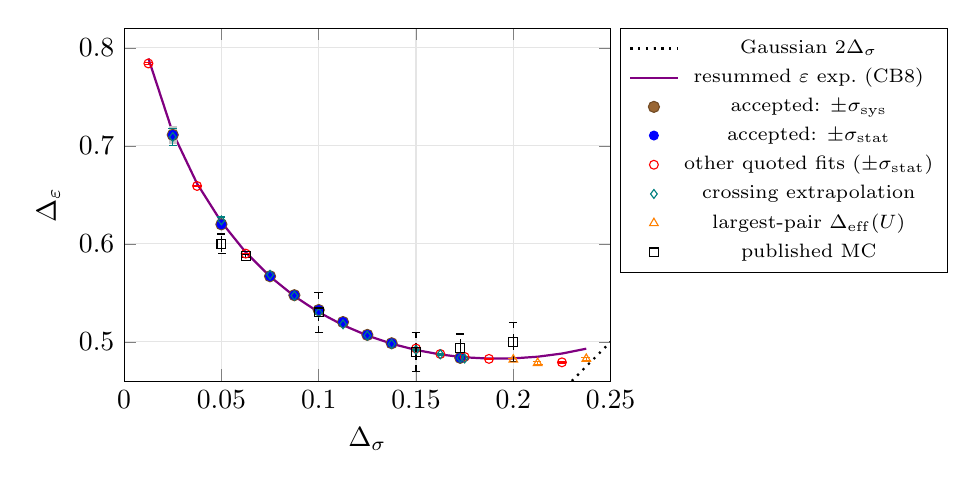
\begin{tikzpicture}
\begin{axis}[width=0.64\textwidth,height=0.5\textwidth,xlabel={$\Delta_\sigma$},ylabel={$\Delta_\varepsilon$},xmin=0,xmax=0.25,ymin=0.46,ymax=0.82,xtick={0,0.05,0.1,0.15,0.2,0.25},scaled x ticks=false,xticklabel style={/pgf/number format/fixed},
 legend style={font=\scriptsize,at={(1.02,1)},anchor=north west},grid=major,grid style={gray!20}]
\addplot[domain=0:0.25,dotted,thick,black] {2*x}; \addlegendentry{Gaussian $2\Delta_\sigma$}
\addplot[thick,violet] coordinates {(0.0125,0.78915) (0.025,0.71343) (0.0375,0.66146) (0.05,0.62223) (0.0625,0.59139) (0.075,0.56663) (0.0875,0.54656) (0.1,0.53025) (0.1125,0.51703) (0.125,0.50643) (0.1375,0.49808) (0.15,0.49171) (0.1625,0.48714) (0.1727335,0.48465) (0.175,0.48424) (0.1875,0.48291) (0.2,0.48312) (0.2125,0.48483) (0.225,0.48808) (0.2375,0.49301)};
\addlegendentry{resummed $\varepsilon$ exp.\ (CB8)}
\addplot+[only marks,mark=none,draw=none,error bars/.cd,y dir=both,y explicit,error bar style={line width=3pt,gray!45},error mark=none] coordinates {(0.025,0.71115) +- (0,0.00959) (0.05,0.61987) +- (0,0.00220) (0.075,0.56694) +- (0,0.00139) (0.0875,0.54761) +- (0,0.00194) (0.1,0.53248) +- (0,0.00242) (0.1125,0.52020) +- (0,0.00217) (0.125,0.50710) +- (0,0.00193) (0.1375,0.49856) +- (0,0.00180) (0.1727335,0.48368) +- (0,0.00078)};
\addlegendentry{accepted: $\pm\sigma_{\rm sys}$}
\addplot+[only marks,mark=*,mark size=1.6pt,blue,error bars/.cd,y dir=both,y explicit] coordinates {(0.025,0.71115) +- (0,0.00049) (0.05,0.61987) +- (0,0.00055) (0.075,0.56694) +- (0,0.00037) (0.0875,0.54761) +- (0,0.00032) (0.1,0.53248) +- (0,0.00020) (0.1125,0.52020) +- (0,0.00025) (0.125,0.50710) +- (0,0.00035) (0.1375,0.49856) +- (0,0.00030) (0.1727335,0.48368) +- (0,0.00052)};
\addlegendentry{accepted: $\pm\sigma_{\rm stat}$}
\addplot+[only marks,mark=o,mark size=1.6pt,red,error bars/.cd,y dir=both,y explicit] coordinates {(0.0125,0.78404) +- (0,0.00077) (0.0375,0.65904) +- (0,0.00051) (0.0625,0.59003) +- (0,0.00035) (0.15,0.49325) +- (0,0.00041) (0.1625,0.48761) +- (0,0.00058) (0.175,0.48460) +- (0,0.00035) (0.1875,0.48263) +- (0,0.00030) (0.225,0.47912) +- (0,0.00068)};
\addlegendentry{other quoted fits ($\pm\sigma_{\rm stat}$)}
\addplot+[only marks,mark=diamond,mark size=1.6pt,teal,error bars/.cd,y dir=both,y explicit] coordinates {(0.025,0.70906) +- (0,0.00902) (0.05,0.62393) +- (0,0.00348) (0.075,0.56843) +- (0,0.00207) (0.0875,0.54711) +- (0,0.00113) (0.1,0.52975) +- (0,0.00135) (0.1125,0.51790) +- (0,0.00086) (0.125,0.50640) +- (0,0.00172) (0.1375,0.49783) +- (0,0.00094) (0.15,0.49183) +- (0,0.00071) (0.1625,0.48732) +- (0,0.00075) (0.1727335,0.48355) +- (0,0.00062) (0.175,0.48304) +- (0,0.00081)};
\addlegendentry{crossing extrapolation}
\addplot+[only marks,mark=triangle,mark size=1.8pt,orange,error bars/.cd,y dir=both,y explicit] coordinates {(0.2,0.4819) +- (0,0.0015) (0.2125,0.4784) +- (0,0.0015) (0.2375,0.4826) +- (0,0.0015)};
\addlegendentry{largest-pair $\Delta_{\rm eff}(U)$}
\addplot+[only marks,mark=square,mark size=1.6pt,black,error bars/.cd,y dir=both,y explicit] coordinates {(0.2,0.5000) +- (0,0.0200) (0.1727335,0.4940) +- (0,0.0140) (0.15,0.4900) +- (0,0.0200) (0.1,0.5300) +- (0,0.0200) (0.0625,0.5876) +- (0,0.0013) (0.05,0.6000) +- (0,0.0100)};
\addlegendentry{published MC}
\end{axis}
\end{tikzpicture}
\caption{$d=1$: $\De(\Ds)$. Values that passed the protocol with $\sstat$ (blue bars) and, separately, the model-family half-range $\ssys$
(gray bands), which is not a standard deviation; other quoted fits; crossing extrapolations with $\sigma_\infty$; largest-pair effective
dimensions where no fit is quotable; published Monte Carlo values; and the resummed $\varepsilon$ expansion. Table~\ref{tab:theory1d} gives the
differences.}\label{fig:1d}
\end{figure}

\paragraph{Reading the results.}
\begin{description}[leftmargin=1.2em]
\item[Near $s\to1$ ($\Ds\le0.05$).] 68--72 configurations are quotable, but $\ssys=4$--$20\times\sstat$: the fitted correction exponents
 ($\omega\approx0.26$--$0.40$) and the variants do not settle the correction sector, as expected near a marginal point.
\item[Middle ($0.0625\le\Ds\le0.1375$).] Six of seven couplings pass, with $\sstat=(2$--$4)\times10^{-4}$ and $\ssys=(1.4$--$2.4)\times10^{-3}$. At
 $\Ds=1/16$ the value is stable across campaigns: 0.59003 (final fit, with N2), 0.59046 (stages A and B alone, under protocol v2) and 0.59071
 (the separate two-point campaign); but the crossing series fail their own goodness-of-fit gate, hence \lbl{cross-check unavailable}.
\item[Towards the Gaussian end ($\Ds\ge0.15$).] $\Ds=0.1727335$ passes. At 0.15 and 0.175 the cross-check fails by $2.1$ and $2.0\sigma_D$; at
 0.1625, 0.1875 and 0.225 only fits of variant \code{second} with $\ktau=2$ are quotable (\lbl{conditional}); at 0.2, 0.2125 and 0.2375 no fit is
 quotable, because the correction exponent $\omega\approx\varepsilon\le0.2$ is too small to separate from the scaling function over $N\le2^{19}$.
 There the finite-size values of table~\ref{tab:1dpairs} are reported; they are not infinite-size estimates.
\end{description}

\subsection{\texorpdfstring{Robustness of the $d=1$ results}{Robustness of the d=1 results}}\label{sec:robust}
Table~\ref{tab:robust} collects, per coupling, the quantities that bear on how much a value or label can be trusted; the paragraphs below
explain them.
\begin{table}[htbp]\centering\scriptsize
\caption{$d=1$ robustness. $n_q$: quotable fits; $P_{\chi^2}$: $\chi^2$ probability of the quoted fit; $\omega$: its correction exponent; fit $-$
crossing: quoted value minus the median crossing extrapolation; $z$: that difference over $\sigma_D$ as pre-registered (with the spread
term) and over the bootstrap part alone; P: label platform-sensitive (section~\ref{sec:1drefit}).}\label{tab:robust}
\begin{tabular}{@{}llrllrrrl@{}}\toprule
$\Ds$ & decision & $n_q$ & $P_{\chi^2}$ & $\omega$ & fit $-$ crossing & $z$ & $z$ (bootstrap) & \\\midrule
0.0125 & \lbl{x-check unavail.} & 72 & 0.01 & 0.262 & -- & -- & -- &  \\
0.025 & \lbl{accepted ($\sigma_{\rm sys}$-dom.)} & 68 & $3.1\times10^{-4}$ & 0.309 & +0.00209 & +0.23 & +0.24 &  \\
0.0375 & \lbl{x-check unavail.} & 71 & 0.21 & 0.348 & -- & -- & -- &  \\
0.05 & \lbl{accepted} & 72 & 0.36 & 0.397 & -0.00406 & -0.92 & -1.16 &  \\
0.0625 & \lbl{x-check unavail.} & 50 & 0.29 & 0.427 & -- & -- & -- &  \\
0.075 & \lbl{accepted} & 30 & 0.51 & 0.418 & -0.00148 & -0.33 & -0.70 &  \\
0.0875 & \lbl{accepted} & 34 & 0.41 & 0.385 & +0.00050 & +0.35 & +0.50 &  \\
0.1 & \lbl{accepted ($\sigma_{\rm sys}$-dom.)} & 48 & $5.2\times10^{-5}$ & 0.367 & +0.00273 & +1.73 & +2.13 &  \\
0.1125 & \lbl{accepted ($\sigma_{\rm sys}$-dom.)} & 41 & $1.5\times10^{-3}$ & 0.368 & +0.00230 & +0.61 & +2.73 &  \\
0.125 & \lbl{accepted} & 9 & $4.6\times10^{-5}$ & 0.368 & +0.00070 & +0.31 & +0.42 &  \\
0.1375 & \lbl{accepted ($\sigma_{\rm sys}$-dom.)} & 17 & 0.03 & 0.365 & +0.00073 & +0.77 & +0.79 &  \\
0.15 & \lbl{x-check failed} & 11 & $2.1\times10^{-3}$ & 0.320 & +0.00143 & +2.10 & +2.24 &  \\
0.1625 & \lbl{conditional} & 5 & 0.05 & 0.194 & +0.00029 & +0.22 & +0.38 & P \\
0.1727335 & \lbl{accepted} & 4 & 0.08 & 0.195 & +0.00013 & +0.17 & +0.20 & P \\
0.175 & \lbl{x-check failed} & 6 & 0.03 & 0.192 & +0.00155 & +2.00 & +2.00 &  \\
0.1875 & \lbl{conditional} & 4 & $1.5\times10^{-4}$ & 0.155 & -- & -- & -- &  \\
0.2 & \lbl{model-limited} & 0 & -- & -- & -- & -- & -- &  \\
0.2125 & \lbl{model-limited} & 0 & -- & -- & -- & -- & -- &  \\
0.225 & \lbl{conditional} & 1 & $7.4\times10^{-4}$ & 0.083 & -- & -- & -- &  \\
0.2375 & \lbl{model-limited} & 0 & -- & -- & -- & -- & -- &  \\
\bottomrule\end{tabular}
\end{table}
\begin{description}[leftmargin=1.2em]
\item[Goodness of fit.] The quality gate $\chi^2/{\rm dof}\le1.5$ admits, at about 200 degrees of freedom, fits with $P_{\chi^2}\sim10^{-5}$.
 The quoted fits at $\Ds=0.1$ and $0.125$ have $P_{\chi^2}\approx5\times10^{-5}$, at 0.025 $P_{\chi^2}=3\times10^{-4}$, and at 0.1125
 $P_{\chi^2}=1.5\times10^{-3}$. The preference for the smallest $N_{\min}$
 selects the member of the family with the most data, which is also often the one with the largest $\chi^2$. For these couplings $\sstat$
 understates the point-to-point scatter, and the values should be read with $\ssys$.
\item[The cross-check and its $\sigma_D$.] Without the spread term in $\sigma_D$ the test would fail at $\Ds=0.1$ ($z=2.13$) and $0.1125$
 ($z=2.73$), both labeled \lbl{accepted}. Moreover, for all nine couplings with $\Ds\ge0.0875$ and a cross-check the fit lies above the
 crossing extrapolation: the inverse-variance mean difference is $+0.00105\pm0.00028$ with $\chi^2=8.1$ for 8 degrees of freedom about it. (Inverse-variance weights from the
 bootstrap part.) The two failures at 0.15 and 0.175 are among the points with the smallest $\sigma_D$, not isolated anomalies. The global fit and the crossings use
 different correction exponents (for example $\omega=0.32$ and $\omega'=0.31$--$0.32$ at 0.15, $\omega=0.19$ and $\omega'=0.27$ at 0.175) and the
 same data, so their comparison is a consistency check of two extrapolation models, not an independent measurement.
\item[The failures and the $\omega'$ grid.] The failures at 0.15 and 0.175 are not an artifact of conditional errors: the crossing bootstrap
 refits $\omega'$ in every draw, and fixing it at its central value would make $\sigma_D$ smaller (table~\ref{tab:oned}). They are, however, numerically fragile:
 refining only the $\omega'$ grid from step 0.01 to 0.001 and 0.0001, with everything else fixed, moves the ratio
 $|\De^{\rm fit}-\De^\infty|/\sigma_D$ from 2.101 to 1.884 and 1.907 at 0.15, and from 2.003 to 1.897 and 1.931 at 0.175, below the
 threshold. The labels stand under the frozen protocol (step 0.01); whether a fit--crossing difference of this size is real is unresolved, and
 the common offset above suggests a systematic difference between the two extrapolation models.
\begin{table}[htbp]\centering\scriptsize
\caption{The cross-check at $\Ds=0.15,0.175$ with $\omega'$ refitted per draw (as recorded) and fixed at its central value. Last column:
central $\omega'$ (16--84\,\% of the per-draw values) of each eligible crossing series.}\label{tab:oned}
\begin{tabular}{@{}llllll>{\raggedright\arraybackslash}p{5.0cm}@{}}\toprule
$\Ds$ & fit $-$ crossing & $\sigma_D$ (per draw) & $z$ & $\sigma_D$ (fixed $\omega'$) & $z$ & series \\\midrule
0.15 & +0.00143 & 0.00068 & +2.10 & 0.00062 & +2.30 & xc0.45\_star: 0.32 (0.31--0.32), xc0.45\_plus: 0.31 (0.30--0.32) \\
0.175 & +0.00155 & 0.00078 & +2.00 & 0.00067 & +2.30 & xc0.6\_star: 0.27 (0.26--0.27), xc0.6\_plus: 0.27 (0.26--0.27) \\
\bottomrule\end{tabular}
\end{table}
\item[Audit.] On 2026-09-22 the second AI system audited the finished analysis, with diagnostic refits
 (no new data) on the same records and bootstrap draws. It found no defect in the sampler, estimators or implementation, and these
 sensitivities:
 \begin{itemize}
 \item The quoted values at $\Ds=0.1$, 0.1375 and 0.1727335 are stable under stronger size cuts ($N\ge32\,768$, $N\ge65\,536$); at
  0.1727335 the cuts give 0.48421 and 0.48386 against 0.48368(52).
 \item At 0.025 a model outside the family (analytic background plus second power together) gives 0.69348, below the family's lower end
  0.69686, a shift of 7.0 paired-bootstrap scales (half the 16--84\,\% width of the matched difference). At 0.175, $N\ge32\,768$ shifts the
  value by $-0.00237$ (2.2 scales); at 0.225, $N\ge65\,536$ shifts it by $+0.00483$ (3.7 scales).
 \item The family is asymmetric: at 0.1375 it extends $0.00020$ below and $0.00340$ above the quoted value.
 \item A regular magnetic background gives an $N^{-s}$ correction to $U$ as well as to $Y$, but the \code{background} variant puts it only on
  $Y$. In the six cases the audit reports (0.025, 0.1, 0.1375, 0.1727335, 0.175, 0.225; variant with background and second power),
  adding it moves the central value by at most 0.0021 (at 0.025). At 0.05 such a model gives 0.61602, 0.0039 below the quoted value and below
  the family range [0.61845, 0.62286] (central fit only, not bootstrapped).
 \end{itemize}
\item[The degree ladder.] In 160 of the 1\,116 configurations, at 15 of the 20 couplings, the ladder cannot take its first step ($p=3$
 against $p=4$) because one of the two fits is missing or flagged. In 140 of them it is the $p=3$ fit, although that fit is typically a gross
 misfit that the F-test would reject by many orders of magnitude; in the other 20 it is the $p=4$ fit. $n_q$ and $\ssys$ are computed on the
 families trimmed in this way. At two couplings this decides the label (section~\ref{sec:1drefit}). A sensitivity study with a ladder
 that does not stop on a flagged lower-degree fit is reported in section~\ref{sec:robustladder}.
\end{description}

\subsubsection{Reproducibility of the fitting stage across platforms}\label{sec:1drefit}
The fit inputs of every coupling (merged summaries and block archives) are released, so the whole fitting stage can be rerun
(\code{make refit1d}). It was rerun for all 20 couplings on 7 October 2026 on a workstation (Intel i9-13900K; Python 3.12.3, NumPy 1.26.4,
SciPy 1.11.4, OpenBLAS) with the production arguments and compared with the production run (AMD EPYC 7742; Python 3.8.5, NumPy 1.19.2, SciPy
1.5.2); table~\ref{tab:refit}. Eighteen labels and all quoted configurations are reproduced, and so is $\ssys$ wherever both runs have it;
quoted values agree to $\le10^{-8}$ and $\sstat$ to $\le1.2\times10^{-7}$ absolute, because nonlinear optima agree only to $\sim10^{-7}$. Two
labels change, in opposite directions, for the same reason: the $p=3$ start of the ladder of configuration \code{x0.45\_background\_Nmin8192\_K2},
a gross misfit ($\chi^2\approx6$--$8\times10^4$ for 178 degrees of freedom, rejected by the F-test at a probability below $10^{-100}$), has two minima, one
interior and a lower one with $a_1$ on its bound $-50$, and which one the multistart optimizer finds depends on floating-point details
(table~\ref{tab:d3}). A bound minimum is flagged and stops the ladder, so the configuration never reaches its good $p\ge5$ fits.
\begin{itemize}
\item At $\Ds=0.1727335$ production found the interior minimum: four quotable fits, $\ssys=0.00078$, \lbl{accepted}. The workstation (with its
 own libraries, and with the production versions in OpenBLAS and MKL builds) and an AMD EPYC 7543 node with the production versions find the
 bound minimum: three fits remain, $\ssys$ needs four, \lbl{conditional}. The fourth fit, which exists only on the production platform, has
 $\chi^2/{\rm dof}=1.47$ against the cap 1.5.
\item At $\Ds=0.1625$ it is the reverse: production found the bound minimum (five quotable fits, all of variant \code{second}, so $\ssys$ is not
 available: \lbl{conditional}); the workstation finds the interior minimum, a sixth fit of variant \code{background} becomes quotable, $\ssys=0.00024$
 and the label is \lbl{accepted}.
\end{itemize}
The values and $\sstat$ are robust; these two labels should be read as platform-sensitive.
\begin{table}[htbp]\centering\scriptsize
\caption{$d=1$ fitting stage rerun from the released snapshots (workstation, 2026-10-07) against production. $n_q$: quotable fits;
$|\delta\De|$: difference of the quoted values. Records: \code{results/1d/refit\_workstation\_20261007/}.}\label{tab:refit}
\begin{tabular}{@{}lllllllll@{}}\toprule
 & \multicolumn{3}{c}{production} & \multicolumn{3}{c}{refit (workstation)} & & \\
$\Ds$ & decision & $n_q$ & $\ssys$ & decision & $n_q$ & $\ssys$ & $|\delta\De|$ & \\\midrule
0.0125 & \lbl{x-check unavail.} & 72 & 0.01003 & \lbl{x-check unavail.} & 72 & 0.01003 & 3e-09 &  \\
0.025 & \lbl{accepted ($\sigma_{\rm sys}$-dom.)} & 68 & 0.00959 & \lbl{accepted ($\sigma_{\rm sys}$-dom.)} & 68 & 0.00959 & 1e-09 &  \\
0.0375 & \lbl{x-check unavail.} & 71 & 0.00425 & \lbl{x-check unavail.} & 71 & 0.00425 & 2e-09 &  \\
0.05 & \lbl{accepted} & 72 & 0.00220 & \lbl{accepted} & 72 & 0.00220 & 5e-09 &  \\
0.0625 & \lbl{x-check unavail.} & 50 & 0.00150 & \lbl{x-check unavail.} & 50 & 0.00150 & 4e-09 &  \\
0.075 & \lbl{accepted} & 30 & 0.00139 & \lbl{accepted} & 30 & 0.00139 & 2e-09 &  \\
0.0875 & \lbl{accepted} & 34 & 0.00194 & \lbl{accepted} & 34 & 0.00194 & 2e-09 &  \\
0.1 & \lbl{accepted ($\sigma_{\rm sys}$-dom.)} & 48 & 0.00242 & \lbl{accepted ($\sigma_{\rm sys}$-dom.)} & 48 & 0.00242 & 8e-10 &  \\
0.1125 & \lbl{accepted ($\sigma_{\rm sys}$-dom.)} & 41 & 0.00217 & \lbl{accepted ($\sigma_{\rm sys}$-dom.)} & 41 & 0.00217 & 2e-09 &  \\
0.125 & \lbl{accepted} & 9 & 0.00193 & \lbl{accepted} & 9 & 0.00193 & 3e-09 &  \\
0.1375 & \lbl{accepted ($\sigma_{\rm sys}$-dom.)} & 17 & 0.00180 & \lbl{accepted ($\sigma_{\rm sys}$-dom.)} & 17 & 0.00180 & 2e-09 &  \\
0.15 & \lbl{x-check failed} & 11 & 0.00306 & \lbl{x-check failed} & 11 & 0.00306 & 2e-10 &  \\
0.1625 & \lbl{conditional} & 5 & -- & \lbl{accepted} & 6 & 0.00024 & 2e-09 & changed \\
0.1727335 & \lbl{accepted} & 4 & 0.00078 & \lbl{conditional} & 3 & -- & 3e-09 & changed \\
0.175 & \lbl{x-check failed} & 6 & 0.00067 & \lbl{x-check failed} & 6 & 0.00067 & 3e-09 &  \\
0.1875 & \lbl{conditional} & 4 & -- & \lbl{conditional} & 4 & -- & 6e-09 &  \\
0.2 & \lbl{model-limited} & 0 & -- & \lbl{model-limited} & 0 & -- & -- &  \\
0.2125 & \lbl{model-limited} & 0 & -- & \lbl{model-limited} & 0 & -- & -- &  \\
0.225 & \lbl{conditional} & 1 & -- & \lbl{conditional} & 1 & -- & 7e-09 &  \\
0.2375 & \lbl{model-limited} & 0 & -- & \lbl{model-limited} & 0 & -- & -- &  \\
\bottomrule\end{tabular}
\end{table}
\begin{table}[htbp]\centering\scriptsize
\caption{The $p=3$ start of the ladder of \code{x0.45\_background\_Nmin8192\_K2} on each platform: $\chi^2$ (178 dof), the field coefficient
$a_1$ (bounds $\pm50$), and the consequence for the ladder.}\label{tab:d3}
\begin{tabular}{@{}llllll@{}}\toprule
$\Ds$ & platform & $\chi^2$ & $a_1$ & minimum & ladder \\\midrule
0.1625 & production (AMD EPYC 7742) & 60656.3 & -50.00 & bound & stops at $p=3$ \\
0.1625 & Intel i9-13900K, Py 3.12/NumPy 1.26/SciPy 1.11, OpenBLAS & 67496.2 & -38.29 & interior & continues \\
0.1727335 & production (AMD EPYC 7742) & 75400.9 & -45.49 & interior & continues \\
0.1727335 & Intel i9-13900K, Py 3.12/NumPy 1.26/SciPy 1.11, OpenBLAS & 68429.4 & -50.00 & bound & stops at $p=3$ \\
0.1727335 & Intel i9-13900K, Py 3.8.5/NumPy 1.19.2/SciPy 1.5.2, OpenBLAS & 68429.4 & -50.00 & bound & stops at $p=3$ \\
0.1727335 & Intel i9-13900K, same versions, MKL & 68429.4 & -50.00 & bound & stops at $p=3$ \\
0.1727335 & AMD EPYC 7543, same versions, MKL & 68429.4 & -50.00 & bound & stops at $p=3$ \\
\bottomrule\end{tabular}
\end{table}

\subsubsection{Sensitivity to the ladder rule}\label{sec:robustladder}
To measure how much the trimmed families matter, all 20 couplings were refitted twice in one job on one node (AMD EPYC 7543; Python 3.8.5,
NumPy 1.19.2, SciPy 1.5.2, MKL): once with the frozen fitter, and once with a copy whose only change is that a flagged lower-degree fit no
longer stops the ladder (its $\chi^2$ still enters the F-test). This is a diagnostic, not the protocol, and table~\ref{tab:1dfinal} is not
modified; records and the modified fitter are in \path{results/1d/robust_ladder_20261013/}. Table~\ref{tab:robustladder} gives the result.
On this node the frozen ladder reproduces the workstation refit of section~\ref{sec:1drefit}, including its two label changes. With the
robust ladder:
\begin{itemize}
\item every quoted value is unchanged to $2\times10^{-5}$;
\item the number of quotable fits grows at eleven couplings, and $\ssys$ grows at 0.125 (0.00193 to 0.00221), 0.1375 (0.00180 to 0.00192), 0.1625
 (0.00024 to 0.00071) and 0.175 (0.00067 to 0.00115);
\item both platform-sensitive couplings pass: 0.1625 with $\ssys=0.00071$, and 0.1727335 with nine quotable fits and the production value
 $\ssys=0.00078$;
\item 0.125 passes as $\ssys$-dominated, 0.1875 becomes \lbl{cross-check unavailable} with $\ssys=0.00063$, and 0.2 becomes \lbl{conditional}
 with two quotable fits.
\end{itemize}
The trimming therefore mostly shrinks the model families; it decides a label only where few fits are quotable. Under the robust rule ten
couplings would pass, and the two platform-sensitive labels would no longer depend on which minimum the degree-3 fit finds.
\begin{table}[htbp]\centering\scriptsize\setlength{\tabcolsep}{3pt}
\caption{$d=1$ ladder sensitivity: production, and the frozen and the robust ladder refitted on one node. $n_q$: quotable fits; $|\delta\De|$:
quoted value, robust minus production; last column: what the robust ladder changes relative to the frozen ladder on the same node.}\label{tab:robustladder}
\begin{tabular}{@{}lllllllllllll@{}}\toprule
 & \multicolumn{3}{c}{production} & \multicolumn{3}{c}{frozen ladder} & \multicolumn{3}{c}{robust ladder} & & \\
$\Ds$ & decision & $n_q$ & $\ssys$ & decision & $n_q$ & $\ssys$ & decision & $n_q$ & $\ssys$ & $|\delta\De|$ & \\\midrule
0.0125 & \lbl{x-check unavail.} & 72 & 0.01003 & \lbl{x-check unavail.} & 72 & 0.01003 & \lbl{x-check unavail.} & 72 & 0.01003 & 1e-09 &  \\
0.025 & \lbl{accepted ($\sigma_{\rm sys}$-dom.)} & 68 & 0.00959 & \lbl{accepted ($\sigma_{\rm sys}$-dom.)} & 68 & 0.00959 & \lbl{accepted ($\sigma_{\rm sys}$-dom.)} & 68 & 0.00959 & 2e-10 &  \\
0.0375 & \lbl{x-check unavail.} & 71 & 0.00425 & \lbl{x-check unavail.} & 71 & 0.00425 & \lbl{x-check unavail.} & 71 & 0.00425 & 9e-10 &  \\
0.05 & \lbl{accepted} & 72 & 0.00220 & \lbl{accepted} & 72 & 0.00220 & \lbl{accepted} & 72 & 0.00220 & 6e-09 &  \\
0.0625 & \lbl{x-check unavail.} & 50 & 0.00150 & \lbl{x-check unavail.} & 50 & 0.00150 & \lbl{x-check unavail.} & 50 & 0.00150 & 3e-09 &  \\
0.075 & \lbl{accepted} & 30 & 0.00139 & \lbl{accepted} & 30 & 0.00139 & \lbl{accepted} & 30 & 0.00139 & 6e-09 &  \\
0.0875 & \lbl{accepted} & 34 & 0.00194 & \lbl{accepted} & 34 & 0.00194 & \lbl{accepted} & 35 & 0.00194 & 2e-09 & $n_q$ \\
0.1 & \lbl{accepted ($\sigma_{\rm sys}$-dom.)} & 48 & 0.00242 & \lbl{accepted ($\sigma_{\rm sys}$-dom.)} & 48 & 0.00242 & \lbl{accepted ($\sigma_{\rm sys}$-dom.)} & 49 & 0.00242 & 1e-10 & $n_q$ \\
0.1125 & \lbl{accepted ($\sigma_{\rm sys}$-dom.)} & 41 & 0.00217 & \lbl{accepted ($\sigma_{\rm sys}$-dom.)} & 41 & 0.00217 & \lbl{accepted ($\sigma_{\rm sys}$-dom.)} & 44 & 0.00217 & 4e-09 & $n_q$ \\
0.125 & \lbl{accepted} & 9 & 0.00193 & \lbl{accepted} & 9 & 0.00193 & \lbl{accepted ($\sigma_{\rm sys}$-dom.)} & 18 & 0.00221 & 2e-05 & label \\
0.1375 & \lbl{accepted ($\sigma_{\rm sys}$-dom.)} & 17 & 0.00180 & \lbl{accepted ($\sigma_{\rm sys}$-dom.)} & 17 & 0.00180 & \lbl{accepted ($\sigma_{\rm sys}$-dom.)} & 24 & 0.00192 & 1e-09 & $n_q$ \\
0.15 & \lbl{x-check failed} & 11 & 0.00306 & \lbl{x-check failed} & 11 & 0.00306 & \lbl{x-check failed} & 19 & 0.00306 & 1e-09 & $n_q$ \\
0.1625 & \lbl{conditional} & 5 & -- & \lbl{accepted} & 6 & 0.00024 & \lbl{accepted} & 15 & 0.00071 & 4e-09 & $n_q$ \\
0.1727335 & \lbl{accepted} & 4 & 0.00078 & \lbl{conditional} & 3 & -- & \lbl{accepted} & 9 & 0.00078 & 2e-09 & label \\
0.175 & \lbl{x-check failed} & 6 & 0.00067 & \lbl{x-check failed} & 6 & 0.00067 & \lbl{x-check failed} & 13 & 0.00115 & 5e-11 & $n_q$ \\
0.1875 & \lbl{conditional} & 4 & -- & \lbl{conditional} & 4 & -- & \lbl{x-check unavail.} & 10 & 0.00063 & 2e-09 & label \\
0.2 & \lbl{model-limited} & 0 & -- & \lbl{model-limited} & 0 & -- & \lbl{conditional} & 2 & -- & -- & label \\
0.2125 & \lbl{model-limited} & 0 & -- & \lbl{model-limited} & 0 & -- & \lbl{model-limited} & 0 & -- & -- &  \\
0.225 & \lbl{conditional} & 1 & -- & \lbl{conditional} & 1 & -- & \lbl{conditional} & 1 & -- & 5e-09 &  \\
0.2375 & \lbl{model-limited} & 0 & -- & \lbl{model-limited} & 0 & -- & \lbl{model-limited} & 0 & -- & -- &  \\
\bottomrule\end{tabular}
\end{table}

\subsection{Comparison with theory and earlier simulations}\label{sec:theory1d}
\paragraph{Resummed $\varepsilon$ expansion.} Table~\ref{tab:theory1d} compares with the eight-loop $\varepsilon$ expansion of the accompanying
article~\cite{Zheng:2026ai}, resummed by conformal Borel resummation~\cite{LeGuillou:1979ixc}. In $d=1$ it is resummed in the variable
$v=1-2\sqrt{\Ds}$, with the short-range series near $s=1$ imposed; we call this curve CB8 (values and band from the article's resummation
package, \path{data/reference/theory_1d_CB8.csv}). The band is a sensitivity range over resummation prescriptions, not a confidence interval.
The nine values that passed the protocol differ from CB8 by $-0.0024$ to $+0.0032$, that is 1 to 13 times their $\sstat$; four of them (0.025,
0.05, 0.1, 0.1125) lie outside the band. As a scale only, $\ssys$ exceeds the difference except at 0.05, 0.1125 and 0.1727335 (1.1, 1.5 and 1.2
times $\ssys$). Near the Gaussian end the series needs little resummation (at $\Ds=0.2375$, $\varepsilon=0.05$, its partial sums are stable to
$3\times10^{-4}$). There the largest-pair effective dimensions (0.2, 0.2125, 0.2375) and the single quoted fit at 0.225 lie $0.0012$,
$0.0065$, $0.0104$ and $0.0090$ below it. A slow approach with exponent $\omega\approx\varepsilon$, which the fit windows and the crossing grid
($\omega'\ge0.2$) cannot resolve, would give a deficit of this sign; we have not estimated its size. These values are finite-size results.
\begin{table}[htbp]\centering\scriptsize
\caption{$d=1$ against the resummed $\varepsilon$ expansion (CB8, with band). MC: the quoted global fit ($\sstat$ only), or the largest-pair
$\Deff(U)$ where no fit is quotable.}\label{tab:theory1d}
\begin{tabular}{@{}llllllll@{}}\toprule
$\Ds$ & $\varepsilon$ & CB8 & band & decision & MC kind & MC & MC $-$ CB8 \\\midrule
0.0125 & 0.950 & 0.7892 & [0.7891, 0.7892] & \lbl{x-check unavail.} & fit & 0.78404(77) & -0.0051 \\
0.025 & 0.900 & 0.7134 & [0.7133, 0.7136] & \lbl{accepted ($\sigma_{\rm sys}$-dom.)} & fit & 0.71115(49) & -0.0023 \\
0.0375 & 0.850 & 0.6615 & [0.6611, 0.6619] & \lbl{x-check unavail.} & fit & 0.65904(51) & -0.0024 \\
0.05 & 0.800 & 0.6222 & [0.6215, 0.6230] & \lbl{accepted} & fit & 0.61987(55) & -0.0024 \\
0.0625 & 0.750 & 0.5914 & [0.5903, 0.5924] & \lbl{x-check unavail.} & fit & 0.59003(35) & -0.0014 \\
0.075 & 0.700 & 0.5666 & [0.5650, 0.5679] & \lbl{accepted} & fit & 0.56694(37) & +0.0003 \\
0.0875 & 0.650 & 0.5466 & [0.5446, 0.5479] & \lbl{accepted} & fit & 0.54761(32) & +0.0011 \\
0.1 & 0.600 & 0.5302 & [0.5280, 0.5316] & \lbl{accepted ($\sigma_{\rm sys}$-dom.)} & fit & 0.53248(20) & +0.0022 \\
0.1125 & 0.550 & 0.5170 & [0.5146, 0.5188] & \lbl{accepted ($\sigma_{\rm sys}$-dom.)} & fit & 0.52020(25) & +0.0032 \\
0.125 & 0.500 & 0.5064 & [0.5040, 0.5086] & \lbl{accepted} & fit & 0.50710(35) & +0.0007 \\
0.1375 & 0.450 & 0.4981 & [0.4958, 0.5005] & \lbl{accepted ($\sigma_{\rm sys}$-dom.)} & fit & 0.49856(30) & +0.0005 \\
0.15 & 0.400 & 0.4917 & [0.4898, 0.4942] & \lbl{x-check failed} & fit & 0.49325(41) & +0.0015 \\
0.1625 & 0.350 & 0.4871 & [0.4857, 0.4895] & \lbl{conditional} & fit & 0.48761(58) & +0.0005 \\
0.1727335 & 0.309 & 0.4846 & [0.4835, 0.4867] & \lbl{accepted} & fit & 0.48368(52) & -0.0010 \\
0.175 & 0.300 & 0.4842 & [0.4832, 0.4862] & \lbl{x-check failed} & fit & 0.48460(35) & +0.0004 \\
0.1875 & 0.250 & 0.4829 & [0.4822, 0.4844] & \lbl{conditional} & fit & 0.48263(30) & -0.0003 \\
0.2 & 0.200 & 0.4831 & [0.4828, 0.4840] & \lbl{model-limited} & largest pair & 0.4819(15) & -0.0012 \\
0.2125 & 0.150 & 0.4848 & [0.4847, 0.4852] & \lbl{model-limited} & largest pair & 0.4784(15) & -0.0065 \\
0.225 & 0.100 & 0.4881 & [0.4881, 0.4882] & \lbl{conditional} & fit & 0.47912(68) & -0.0090 \\
0.2375 & 0.050 & 0.4930 & [0.4930, 0.4930] & \lbl{model-limited} & largest pair & 0.4826(15) & -0.0104 \\
\bottomrule\end{tabular}
\end{table}

\paragraph{Earlier simulations.} Table~\ref{tab:lit1d} lists the published Monte Carlo values at our couplings (earlier estimates from exact
finite-range scaling~\cite{Glumac:1989fr} are not simulations and are not listed). Published values exist at
six of our couplings; at three of them (0.05, 0.1, 0.1727335) our value passed the protocol, and at $\Ds=0.2$ the comparison is with a finite-size
value. The equilibrium values (UGA, APR, Luijten's thesis) agree with ours to within two standard deviations of the difference, computed from the
published error and our $\sstat$; $\ssys$ is not added, because it is not a standard deviation. The largest ratio, 1.98, is at $\Ds=0.05$,
where the difference is nine times our $\ssys$. The nonequilibrium-relaxation values of Tomita lie below; his own estimate of $\eta$
misses the exact $\eta=2-s$ by 2.5--3.5 quoted errors at $s=0.6$--$0.8$, so his quoted errors do not cover the systematic errors of that
method, and the disagreement at $\Ds=0.1$ is with an estimate that fails an exact check. APR's correction exponent $\omega=0.201(11)$ at
$\Ds=0.1727335$ agrees with our fitted $\omega=0.195$ (table~\ref{tab:robust}).
\begin{table}[htbp]\centering\scriptsize
\caption{Published $d=1$ values ($\De=1-1/\nu$ where $\nu$ is quoted) against ours. UGA: Uzelac--Glumac--Ani\v{c}i\'c; APR: Angelini--Parisi--Ricci-Tersenghi; NER: nonequilibrium relaxation. Ours: value($\sstat$)($\ssys$), or a finite-size value.}\label{tab:lit1d}
\setlength{\tabcolsep}{2.5pt}\begin{tabular}{@{}lllllll@{}}\toprule
$\Ds$ & source & method & published & ours & our label & published $-$ ours \\\midrule
0.05 & Tomita 2009~\cite{Tomita:2009mc} & MC, NER & 0.5633(362) & 0.61987(55)(220) & \lbl{accepted} & -0.0566 \\
0.05 & UGA 2001~\cite{Uzelac:2001lc} & MC, largest cluster & 0.6000(100) & 0.61987(55)(220) & \lbl{accepted} & -0.0199 \\
0.0625 & APR 2014~\cite{Angelini:2014koy} & MC, FSS & 0.5876(13) & 0.59003(35)(150) & \lbl{x-check unavail.} & -0.0024 \\
0.1 & Luijten 1997 (thesis)~\cite{Luijten:1997th} & MC, FSS & 0.5392(106) & 0.53248(20)(242) & \lbl{accepted ($\sigma_{\rm sys}$-dom.)} & +0.0067 \\
0.1 & Tomita 2009~\cite{Tomita:2009mc} & MC, NER & 0.4709(140) & 0.53248(20)(242) & \lbl{accepted ($\sigma_{\rm sys}$-dom.)} & -0.0616 \\
0.1 & UGA 2001~\cite{Uzelac:2001lc} & MC, largest cluster & 0.5300(200) & 0.53248(20)(242) & \lbl{accepted ($\sigma_{\rm sys}$-dom.)} & -0.0025 \\
0.15 & Tomita 2009~\cite{Tomita:2009mc} & MC, NER & 0.4536(508) & 0.49325(41)(306) & \lbl{x-check failed} & -0.0397 \\
0.15 & UGA 2001~\cite{Uzelac:2001lc} & MC, largest cluster & 0.4900(200) & 0.49325(41)(306) & \lbl{x-check failed} & -0.0033 \\
0.1727335 & APR 2014~\cite{Angelini:2014koy} & MC, FSS & 0.4940(140) & 0.48368(52)(78) & \lbl{accepted} & +0.0103 \\
0.2 & Tomita 2009~\cite{Tomita:2009mc} & MC, NER & 0.4444(648) & 0.4819(15) [finite size] & \lbl{model-limited} & -0.0375 \\
0.2 & UGA 2001~\cite{Uzelac:2001lc} & MC, largest cluster & 0.5000(200) & 0.4819(15) [finite size] & \lbl{model-limited} & +0.0181 \\
\bottomrule\end{tabular}
\end{table}

\subsection{Status of the design goals}
The campaign had three design goals: \lbl{accepted} at every $\Ds\in[0.0625,0.1875]$, which was not met (7 of 12 couplings); a definite label
at every outer coupling, which was met; and exact reproduction of the two-point campaign's values in its original windows, which was met. An
extension to $N=2^{20}$ (called N3) was not run.

% =====================================================================================================================
\section{\texorpdfstring{$d=2$ and $d=3$: common protocol}{d=2 and d=3: common protocol}}\label{sec:proto23}
\subsection{Design and analysis}
For each coupling, five sizes form four size-doubling pairs, the minimum for an extrapolation with a free exponent. Temperatures are centered
on crossings measured in a short stage-0 campaign (frozen tables \path{data/2d/production_centers.csv},
\path{data/3d/production_centers_3d.csv}), five per size. Every $(L,\beta)$ group has 12 hot/cold replicas with $10^6$ measured sweeps; each
dimension has 2\,400 chains.
\begin{enumerate}[1.]
\item For each pair and $Q\in\{U_4,U_6,U_8,Y\}$ the effective dimension~\eqref{eq:Deff} is computed at the $U_4$ crossing; the bootstrap gives
 the covariance over pairs and observables.
\item Each series $\Deff^Q(L)$ is extrapolated as $\De+c_QL^{-\omega'}$ by generalized least squares, with $\omega'$ profiled on $[0.2,2]$ (step
 0.01); a \emph{joint} series fits $U_4$ and $Y$ with common $\De$ and $\omega'$ and separate amplitudes (written U4+Y).
\item A series is eligible if $\chi^2/{\rm dof}\le2$, its $\Delta\chi^2\le1$ interval of $\omega'$ lies inside $[0.22,1.98]$, and its
 $\sigma_\infty$ is at most 5 times the error of the largest pair.
\item The quoted value is that of the joint series if eligible, else $U_4$, else the first eligible one of $U_6$, $U_8$, $Y$; $\ssys$ is half
 the range of $\De$ over the eligible series plus half the range of the quoted series' $\De$ over its $\Delta\chi^2\le1$ interval of $\omega'$.
\item Cross-check: the extrapolated $U_4$ and $Y$ must agree within $2\sigma_D$; reblocking at blocks 1000 and 4000 against 2000.
\end{enumerate}
The grid floor $\omega'\ge0.2$ excludes the correction exponent expected near the Gaussian end ($\omega\approx\varepsilon=0.1$ at 2D $s=1.05$
and 3D $s=1.55$), and near the short-range end the relevant exponent $s_*-s$ is also below 0.2; there the labels partly reflect this design
choice.

\subsection{The statistical error of an extrapolation: amendment P1}\label{sec:p1}
The frozen protocols compute $\sstat$, $\sigma_D$ and the reblocking comparison by refitting each bootstrap draw at the \emph{central}
$\omega'$, i.e.\ conditionally on a fitted exponent. A review of the finished evaluations identified this. Amendment P1
re-profiles $\omega'$ in every draw (same grid and covariance; draws on a grid edge are kept). It leaves the eligibility gates, $\ssys$, the
choice of series and the decision order unchanged. The gate $\sigma_\infty\le5\times$ (error of the largest pair) is therefore still evaluated
with the fixed-$\omega'$ $\sigma_\infty$. With the profiled one, three series would fail it: $Y$ at 2D $s=1.05$ and $U_4$ at 3D $s=1.55$ and
1.7. 2D $s=1.05$ would then have no eligible series, and the 3D cross-check would become unavailable at 1.55 and 1.7. The series of the
accepted value at 3D $s=1.6$ pass the gate either way.

P1 was calibrated before adoption on synthetic data whose truths are the recorded fits: for every coupling, single-series ensembles for each
of $U_4,U_6,U_8,Y$ and a joint ensemble, 2\,000 synthetic data sets each with 500 synthetic draws, run through the full fit, gates and both error
rules. A coupling is evaluated under P1 only if every series it uses has profiled $1\sigma$ coverage $\ge0.60$ and $2\sigma$ coverage $\ge0.90$
(with at least 200 eligible fits) and, when both $U_4$ and $Y$ are eligible, the profiled cross-check's false-failure rate is $\le0.10$;
otherwise the frozen rule applies (appendix~\ref{app:calib}).

Results:
\begin{itemize}
\item The fixed-$\omega'$ rule under-covers mainly for single series: in the strata that pass the adoption rules its $1\sigma$ coverage is
 0.00--0.38 for $U_4$ and 0.12--0.29 for $Y$, against 0.59--0.67 for the joint series (pooled over all strata, the $1\sigma$ coverage is 0.287 for
45\,440 eligible synthetic fits). In the same
 strata the profiled rule covers 0.81--1.00 for the Binder series, 0.69--0.83 for $Y$ and 0.67--0.70 for the joint series.
\item The false-failure rate of the cross-check at 3D $s=1.6$ is 0.7\,\% profiled against 61\,\% fixed.
\end{itemize}
The calibration is \emph{conditional on the single-power model}. We tested one misspecified family, which adds an $L^{-2\omega'}$ term that
reproduces the recorded $U_4-Y$ difference. In it the joint series at 3D $s=1.6$ is biased by $-0.0062$ with profiled coverage 0, and the
profiled cross-check does not detect the bias. But $U_4$ is then ineligible in every synthetic set, so that coupling could not have been
accepted under this misspecification.
The calibration therefore does not test model errors; the one misspecification studied would have blocked the label rather than biased it.
Exactly one label changes under P1: 3D $s=1.6$, from \lbl{cross-check failed} to \lbl{accepted}. This was predicted before implementation, but
after the frozen $z=-2.87$ was known.

% =====================================================================================================================
\section{\texorpdfstring{$d=2$}{d=2}}\label{sec:2d}
Couplings $s\in\{1.05,\dots,1.7\}$ ($\Ds=0.475\dots0.15$), sizes $L=64\dots1024$, temperature half-width $w(L)=0.0015(L/64)^{-0.75}$. Stage 0 used
$L\le512$; the preflight confirmed every $512\to1024$ crossing inside its bracket. The production ran on 2026-09-20 to 22 ($L=1024$ at 88~ms per
sweep, 25--31~h per chain).
\begin{sidewaystable}\centering\scriptsize
\caption{$d=2$ finite-size data (block 2000): for each doubling pair the crossing inverse temperature $\beta_\times$ (error in units of $10^{-7}$) and
$\Deff(U_4)$, $\Deff(Y)$ (errors in units of $10^{-4}$, 500 bootstrap draws).}\label{tab:2dpairs}
\begin{tabular}{@{}ll|lll|lll|lll|lll@{}}\toprule
 & & \multicolumn{3}{c|}{$64\to128$} & \multicolumn{3}{c|}{$128\to256$} & \multicolumn{3}{c|}{$256\to512$} & \multicolumn{3}{c}{$512\to1024$}\\
$s$ & $\Ds$ & $\beta_\times$ & $U_4$ & $Y$ & $\beta_\times$ & $U_4$ & $Y$ & $\beta_\times$ & $U_4$ & $Y$ & $\beta_\times$ & $U_4$ & $Y$ \\\midrule
1.05 & 0.475 & 0.1300733(16) & 0.9633(13) & 0.8390(14) & 0.1300298(10) & 0.9661(17) & 0.8658(18) & 0.1300145(6) & 0.9708(20) & 0.8863(21) & 0.1300084(4) & 0.9702(25) & 0.8964(23) \\
1.1 & 0.45 & 0.1355249(16) & 0.9609(14) & 0.8608(15) & 0.1354801(10) & 0.9639(17) & 0.8912(18) & 0.1354691(6) & 0.9664(20) & 0.9045(19) & 0.1354627(4) & 0.9659(23) & 0.9172(23) \\
1.2 & 0.4 & 0.1463564(17) & 0.9610(12) & 0.9142(13) & 0.1463343(10) & 0.9576(16) & 0.9281(16) & 0.1463269(5) & 0.9616(19) & 0.9391(19) & 0.1463241(3) & 0.9631(22) & 0.9478(22) \\
1.3 & 0.35 & 0.1571230(17) & 0.9581(12) & 0.9561(12) & 0.1571157(9) & 0.9586(15) & 0.9683(15) & 0.1571170(6) & 0.9605(17) & 0.9709(18) & 0.1571177(3) & 0.9584(20) & 0.9698(20) \\
1.4 & 0.3 & 0.1677986(17) & 0.9599(12) & 1.0024(12) & 0.1678175(9) & 0.9590(14) & 1.0032(14) & 0.1678263(5) & 0.9582(17) & 0.9986(16) & 0.1678310(3) & 0.9627(20) & 0.9977(19) \\
1.5 & 0.25 & 0.1783705(17) & 0.9608(12) & 1.0484(11) & 0.1784129(10) & 0.9615(14) & 1.0423(13) & 0.1784331(5) & 0.9640(16) & 1.0339(15) & 0.1784417(3) & 0.9661(18) & 1.0245(17) \\
1.6 & 0.2 & 0.1888074(18) & 0.9653(12) & 1.0977(11) & 0.1888717(10) & 0.9652(13) & 1.0885(12) & 0.1889039(5) & 0.9691(15) & 1.0729(13) & 0.1889149(3) & 0.9698(18) & 1.0620(15) \\
1.7 & 0.15 & 0.1990663(19) & 0.9671(11) & 1.1516(10) & 0.1991553(10) & 0.9699(13) & 1.1381(11) & 0.1991952(5) & 0.9751(16) & 1.1254(14) & 0.1992121(3) & 0.9773(17) & 1.1088(14) \\
\bottomrule\end{tabular}
\end{sidewaystable}
\begin{table}[htbp]\centering\scriptsize
\caption{$d=2$ labels under the frozen rule and under P1 (with the rule actually applied), the quoted value, $\sstat$ under both rules,
$\ssys$, and the $U_4-Y$ cross-check ($z$ with the fixed and the profiled $\sigma_D$). The \lbl{conditional} values at $s=1.05$ and $1.1$ are
single-series ($Y$) extrapolations $0.065$ and $0.047$ below the resummed expansion (table~\ref{tab:theory23}); they are not infinite-size
estimates.}\label{tab:2ddec}
\setlength{\tabcolsep}{4pt}\begin{tabular}{@{}llllllllll@{}}\toprule
$s$ & $\Ds$ & frozen label & P1 label & rule & $\De$ & $\sstat$ frozen & $\sstat$ P1 & $\ssys$ & $U_4-Y$; $z$ fixed / profiled \\\midrule
1.05 & 0.475 & \lbl{conditional} & \lbl{conditional} & profiled & 0.92078 & 0.00181 & 0.01773 & -- & -- \\
1.1 & 0.45 & \lbl{conditional} & \lbl{conditional} & profiled & 0.92846 & 0.00145 & 0.01012 & -- & -- \\
1.2 & 0.4 & \lbl{conditional} & \lbl{conditional} & profiled & 0.96202 & 0.00162 & 0.00182 & -- & -- \\
1.3 & 0.35 & \lbl{model-limited} & \lbl{model-limited} & fixed & -- & -- & -- & -- & -- \\
1.4 & 0.3 & \lbl{model-limited} & \lbl{model-limited} & fixed & -- & -- & -- & -- & -- \\
1.5 & 0.25 & \lbl{model-limited} & \lbl{model-limited} & fixed & -- & -- & -- & -- & -- \\
1.6 & 0.2 & \lbl{model-limited} & \lbl{model-limited} & fixed & -- & -- & -- & -- & -- \\
1.7 & 0.15 & \lbl{model-limited} & \lbl{model-limited} & fixed & -- & -- & -- & -- & -- \\
\bottomrule\end{tabular}
\end{table}

\paragraph{Reading.} No 2D coupling has a value that passed the protocol. The robust statement is finite-size: $\Deff(U_4,512\to1024)=0.958$--$0.977$
at all eight couplings ($\sigma\approx0.002$), moving by $\le0.01$ over the four pairs and always below the endpoint value 1. Against the
resummed expansion (table~\ref{tab:theory23}) the largest-pair $U_4$ agrees within $0.0015$ for $s=1.2$--$1.4$ and falls short by $0.005$--$0.02$
towards both ends. At $s=1.2$, 1.3 and 1.4 the other ways of imposing the end point move the expansion by up to $0.0005$, $0.0023$ and $0.0047$,
so there the agreement is as good as the expansion is determined. $Y$ approaches $U_4$ as $L$ doubles at every coupling, slowly and from below at $s\le1.2$ and from above at $s\ge1.4$; near $s_*$ this is
consistent with the slow crossover of section~\ref{sec:model}. A single power $L^{-\omega'}$ with $\omega'\in[0.2,2]$ is either unresolved or inconsistent over $L=64$--$1024$
(appendix~\ref{app:series}). The three \lbl{conditional} values rest on one series without $\ssys$; at $s=1.05$ and $1.1$ that series is $Y$, and
its extrapolations (0.921, 0.928) lie $0.065$ and $0.047$ below the expansion, 3.7 and 4.6 times their $\sstat$. \textbf{These two values should
not be used as infinite-size estimates.} The crossing inverse temperatures $\beta_\times$ still move by up to $1.7\times10^{-5}$ between the last two
pairs; they are finite-size values.

% =====================================================================================================================
\section{\texorpdfstring{$d=3$}{d=3}}\label{sec:3d}
Couplings $s\in\{1.55,\dots,1.95\}$ ($\Ds=0.725\dots0.525$), sizes $L=8\dots128$, half-width $w(L)=10^{-3}(L/16)^{-1}$. An $L=128$ chain runs at
105~ms per sweep alone but at about 250~ms when four chains share a 4-core CCX (a group of cores sharing a 16~MB L3 cache); the production
therefore pinned one $L=128$ chain per CCX (32 per 128-core node, $\approx30$~h per chain). The preflight gate and its amendment are described in
section~\ref{sec:rules}. The production ran on 2026-09-21 to 23.
\begin{sidewaystable}\centering\scriptsize
\caption{$d=3$ finite-size data (block 2000), as table~\ref{tab:2dpairs}.}\label{tab:3dpairs}
\begin{tabular}{@{}ll|lll|lll|lll|lll@{}}\toprule
 & & \multicolumn{3}{c|}{$8\to16$} & \multicolumn{3}{c|}{$16\to32$} & \multicolumn{3}{c|}{$32\to64$} & \multicolumn{3}{c}{$64\to128$}\\
$s$ & $\Ds$ & $\beta_\times$ & $U_4$ & $Y$ & $\beta_\times$ & $U_4$ & $Y$ & $\beta_\times$ & $U_4$ & $Y$ & $\beta_\times$ & $U_4$ & $Y$ \\\midrule
1.55 & 0.725 & 0.0894786(14) & 1.4427(11) & 1.2535(12) & 0.0893412(7) & 1.4583(15) & 1.3545(16) & 0.0893146(4) & 1.4677(22) & 1.4028(23) & 0.0893087(2) & 1.4729(30) & 1.4269(30) \\
1.6 & 0.7 & 0.0916831(15) & 1.4398(11) & 1.2914(13) & 0.0915467(8) & 1.4596(15) & 1.3970(17) & 0.0915234(4) & 1.4661(21) & 1.4382(23) & 0.0915178(2) & 1.4715(31) & 1.4628(30) \\
1.7 & 0.65 & 0.0959967(15) & 1.4411(11) & 1.3761(12) & 0.0958738(8) & 1.4528(16) & 1.4673(17) & 0.0958528(3) & 1.4612(22) & 1.5085(21) & 0.0958497(2) & 1.4650(29) & 1.5263(29) \\
1.75 & 0.625 & 0.0981147(16) & 1.4377(11) & 1.4115(12) & 0.0979933(8) & 1.4535(15) & 1.5071(16) & 0.0979751(3) & 1.4536(21) & 1.5379(21) & 0.0979722(2) & 1.4615(27) & 1.5596(27) \\
1.8 & 0.6 & 0.1002020(16) & 1.4372(11) & 1.4513(12) & 0.1000841(8) & 1.4505(14) & 1.5417(15) & 0.1000677(3) & 1.4563(20) & 1.5795(20) & 0.1000665(2) & 1.4515(27) & 1.5818(27) \\
1.85 & 0.575 & 0.1022550(15) & 1.4364(11) & 1.4929(12) & 0.1021468(8) & 1.4490(15) & 1.5776(16) & 0.1021325(3) & 1.4538(20) & 1.6113(20) & 0.1021317(2) & 1.4569(27) & 1.6221(27) \\
1.9 & 0.55 & 0.1042865(17) & 1.4370(10) & 1.5325(12) & 0.1041795(8) & 1.4458(14) & 1.6148(15) & 0.1041684(4) & 1.4526(19) & 1.6464(20) & 0.1041687(2) & 1.4511(26) & 1.6488(25) \\
1.95 & 0.525 & 0.1062845(16) & 1.4320(11) & 1.5694(11) & 0.1061853(7) & 1.4466(15) & 1.6539(15) & 0.1061755(4) & 1.4481(20) & 1.6771(21) & 0.1061771(2) & 1.4493(28) & 1.6790(27) \\
\bottomrule\end{tabular}
\end{sidewaystable}
\begin{table}[htbp]\centering\scriptsize
\caption{$d=3$ labels, as table~\ref{tab:2ddec}. At $s=1.7$ and $1.85$ P1 is not calibrated (rule ``fixed'', appendix~\ref{app:calib}): the
profiled $z$ is shown for information only, and the label uses the fixed $z$. The extrapolated values at $s=1.7$--$1.9$ lie $0.022$--$0.033$
above the resummed expansion (table~\ref{tab:theory23}).}\label{tab:3ddec}
\setlength{\tabcolsep}{4pt}\begin{tabular}{@{}llllllllll@{}}\toprule
$s$ & $\Ds$ & frozen label & P1 label & rule & $\De$ & $\sstat$ frozen & $\sstat$ P1 & $\ssys$ & $U_4-Y$; $z$ fixed / profiled \\\midrule
1.55 & 0.725 & \lbl{x-check failed} [$\sigma$] & \lbl{x-check failed} [$\sigma$] & profiled & 1.48118 & 0.00165 & 0.01632 & 0.02716 & +0.0326; +29.48 / +2.49 \\
1.6 & 0.7 & \lbl{x-check failed} [$\sigma$] & \lbl{accepted} [$\sigma$] & profiled & 1.47314 & 0.00112 & 0.00118 & 0.00230 & -0.0025; -2.87 / -0.45 \\
1.7 & 0.65 & \lbl{x-check failed} & \lbl{x-check failed} & fixed & 1.47375 & 0.00174 & 0.00174 & 0.05237 & -0.0676; -56.57 / -4.90 \\
1.75 & 0.625 & \lbl{model-limited} & \lbl{model-limited} & fixed & -- & -- & -- & -- & -- \\
1.8 & 0.6 & \lbl{model-limited} & \lbl{model-limited} & fixed & -- & -- & -- & -- & -- \\
1.85 & 0.575 & \lbl{x-check failed} & \lbl{x-check failed} & fixed & 1.45830 & 0.00103 & 0.00103 & 0.09064 & -0.1723; -232.64 / -28.05 \\
1.9 & 0.55 & \lbl{x-check unavail.} & \lbl{x-check unavail.} & profiled & 1.45449 & 0.00113 & 0.00720 & 0.00452 & -- \\
1.95 & 0.525 & \lbl{model-limited} & \lbl{model-limited} & fixed & -- & -- & -- & -- & -- \\
\bottomrule\end{tabular}
\end{table}

\paragraph{The value at $s=1.6$.} At $s=1.6$ ($\Ds=0.70$) all five series are eligible: $U_4$ 1.4726, $U_6$ 1.4720, $U_8$ 1.4709, $Y$ 1.4750, U4+Y
1.4731. The quoted value comes from the joint series: $\De=1.47314\pm0.00118\,(\mathrm{stat})\pm0.00230\,(\mathrm{sys})$ ($\omega'=1.24$,
$\chi^2=2.38/4$); the range over the $U_4$ and $Y$ series alone is 1.4726--1.4750. It passed the protocol only under amendment P1, and the
precision suffix remains ($\sigma=0.0031>0.003$ at $64\to128$). Three facts limit what the label shows. The cross-check has little power here:
the extrapolated $Y-U_4$ changes sign between $s=1.55$ and $1.7$ ($-0.033$, $+0.002$, $+0.068$), so their agreement at 1.6 is partly a crossing of
two biased estimates, and the profiled $\sigma_D\approx0.0055$ cannot test a $\sstat$ of 0.0012. The fitted $\omega'=1.24$ is far above the
leading exponents expected at $s=1.6$ ($\omega\approx\varepsilon\approx0.2$; $s_*-s\approx0.36$), so the single power is an effective
description. And the label changed under an amendment adopted after the frozen result was known. The value is \emph{consistent} with the
resummed expansion (1.4721) and with the finite-size $\Deff(U_4,64\to128)=1.4715(31)$, which is the main reason to trust it.

\paragraph{Reading.} The finite-size $U_4$ exponent at $64\to128$ decreases from 1.473 ($s=1.55$) to 1.449 ($s=1.95$), between the Gaussian value
1.5 and the short-range value 1.4126. $Y$ does not converge towards $U_4$ at $s\ge1.7$: it lies above $U_4$ from $16\to32$ on and keeps rising
(1.53--1.68 at $64\to128$). Against the resummed expansion (table~\ref{tab:theory23}), the extrapolated values at $s=1.7$--$1.9$ lie
$0.022$--$0.033$ above. At 1.7 and 1.85 the label is \lbl{cross-check failed}, and the differences ($+0.022$, $+0.030$) are smaller than $\ssys$
(0.052, 0.091), which is large because the series disagree; at 1.9 (\lbl{cross-check unavailable}, $\ssys=0.0045$) the difference is 4.6
times $\sstat$. Near $s_*$ the $U_4$ series therefore sits high, and the $Y$--$U_4$
split matches in size the slow crossover of section~\ref{sec:model} at the largest pair, although its growth with $L$ up to 128 is not
reproduced by that leading-order picture.

\subsection{\texorpdfstring{$d=2,3$ against theory and earlier work}{d=2,3 against theory and earlier work}}
Table~\ref{tab:theory23} compares with CB8 and figure~\ref{fig:23} shows the effective dimensions. Table~\ref{tab:lit23} lists published values
inside the window. In $d=2$ the Monte Carlo values (APR, Luijten's thesis, Picco) have errors 0.02--0.034 and differ from our largest-pair
$\Deff(U_4)$ by at most two of their errors; they do not distinguish our finite-size values from CB8. In $d=3$, at $s=1.6$, Luijten's
$L\le64$ values (1.477(16), 1.500(20)) and the functional-RG value (1.475) lie 0.002--0.027 above our accepted value, within 1.3 of their
errors. Nearer $s_*$ the bootstrap values agree with CB8 to about 0.01 or lie slightly below it, while the functional-RG values are close to
our largest-pair $\Deff(U_4)$, up to 0.03 above CB8 (both read off figures). Published values at the ends of the window, $s=d/2$ in
$d=3$~\cite{Luijten:1997cl} and $s=s_*$ in $d=2$~\cite{Xiao:2025sk}, are in the reference files but outside our grid.
\begin{table}[htbp]\centering\scriptsize
\caption{$d=2$ (top) and $d=3$ (bottom) against the resummed $\varepsilon$ expansion of the accompanying article (CB8, with band;
\code{data/reference/theory\_2d3d\_CB8.csv}). CB8 imposes the short-range end: in $d=2$ the value 1, zero slope and the curvature, in $d=3$
the value and the slope $0.27315$, itself an estimate (range 0.269--0.276). The band is a sensitivity range over prescriptions; it excludes
the way the end point is imposed, which in $d=2$ moves the curve by up to 0.0005, 0.0023, 0.0047, 0.0057, 0.0070 and 0.0055 at
$s=1.2,\dots,1.7$, and the 3D slope range. Last two columns: quoted value minus CB8, and largest-pair $\Deff(U_4)$ minus CB8.}\label{tab:theory23}
\setlength{\tabcolsep}{4.5pt}\begin{tabular}{@{}llllllllll@{}}\toprule
$s$ & P1 label & $\De$ & $\sstat$ & $\ssys$ & $\Deff(U_4)$ largest pair & CB8 & band & $\De-$CB8 & $U_4-$CB8 \\\midrule
1.05 & \lbl{conditional} & 0.92078 & 0.01773 & -- & 0.9702(25) & 0.9858 & [0.9858, 0.9858] & -0.0651 & -0.0157 \\
1.1 & \lbl{conditional} & 0.92846 & 0.01012 & -- & 0.9659(23) & 0.9754 & [0.9753, 0.9754] & -0.0470 & -0.0095 \\
1.2 & \lbl{conditional} & 0.96202 & 0.00182 & -- & 0.9631(22) & 0.9626 & [0.9609, 0.9628] & -0.0005 & +0.0006 \\
1.3 & \lbl{model-limited} & -- & -- & -- & 0.9584(20) & 0.9581 & [0.9546, 0.9589] & -- & +0.0003 \\
1.4 & \lbl{model-limited} & -- & -- & -- & 0.9627(20) & 0.9612 & [0.9572, 0.9624] & -- & +0.0015 \\
1.5 & \lbl{model-limited} & -- & -- & -- & 0.9661(18) & 0.9711 & [0.9684, 0.9722] & -- & -0.0050 \\
1.6 & \lbl{model-limited} & -- & -- & -- & 0.9698(18) & 0.9854 & [0.9845, 0.9858] & -- & -0.0157 \\
1.7 & \lbl{model-limited} & -- & -- & -- & 0.9773(17) & 0.9978 & [0.9977, 0.9978] & -- & -0.0205 \\
\midrule
1.55 & \lbl{x-check failed} [$\sigma$] & 1.48118 & 0.01632 & 0.02716 & 1.4729(30) & 1.4849 & [1.4849, 1.4849] & -0.0037 & -0.0119 \\
1.6 & \lbl{accepted} [$\sigma$] & 1.47314 & 0.00118 & 0.00230 & 1.4715(31) & 1.4721 & [1.4721, 1.4721] & +0.0010 & -0.0006 \\
1.7 & \lbl{x-check failed} & 1.47375 & 0.00174 & 0.05237 & 1.4650(29) & 1.4515 & [1.4515, 1.4516] & +0.0222 & +0.0134 \\
1.75 & \lbl{model-limited} & -- & -- & -- & 1.4615(27) & 1.4430 & [1.4429, 1.4431] & -- & +0.0185 \\
1.8 & \lbl{model-limited} & -- & -- & -- & 1.4515(27) & 1.4352 & [1.4352, 1.4353] & -- & +0.0163 \\
1.85 & \lbl{x-check failed} & 1.45830 & 0.00103 & 0.09064 & 1.4569(27) & 1.4281 & [1.4280, 1.4281] & +0.0302 & +0.0288 \\
1.9 & \lbl{x-check unavail.} & 1.45449 & 0.00720 & 0.00452 & 1.4511(26) & 1.4212 & [1.4212, 1.4213] & +0.0333 & +0.0299 \\
1.95 & \lbl{model-limited} & -- & -- & -- & 1.4493(28) & 1.4145 & [1.4145, 1.4145] & -- & +0.0348 \\
\bottomrule\end{tabular}
\end{table}
\begin{table}[htbp]\centering\scriptsize
\caption{Published values inside the long-range window, $d=2$ (top) and $d=3$ (bottom), with our largest-pair $\Deff(U_4)$ and CB8 where the
coupling is on our grid. Bootstrap and functional-RG values are read off figures.}\label{tab:lit23}
\begin{tabular}{@{}lllllll@{}}\toprule
$s$ & source & method & $L_{\max}$ & $\De$ & our $\Deff(U_4)$ & CB8 \\\midrule
1.2 & APR 2014~\cite{Angelini:2014koy} & Monte Carlo & -- & 0.976(34) & 0.9631(22) & 0.9626 \\
1.2 & Luijten thesis 1997~\cite{Luijten:1997th}, Tab.~5.7 & Monte Carlo & 400 & 1.000(20) & 0.9631(22) & 0.9626 \\
1.2 & Luijten thesis 1997~\cite{Luijten:1997th}, Tab.~5.8 & Monte Carlo & 400 & 0.980(30) & 0.9631(22) & 0.9626 \\
1.30906 & APR 2014~\cite{Angelini:2014koy} & Monte Carlo & -- & 0.986(33) & -- & -- \\
1.4 & Luijten thesis 1997~\cite{Luijten:1997th}, Tab.~5.7 & Monte Carlo & 400 & 1.000(20) & 0.9627(20) & 0.9612 \\
1.4 & Luijten thesis 1997~\cite{Luijten:1997th}, Tab.~5.8 & Monte Carlo & 400 & 0.960(30) & 0.9627(20) & 0.9612 \\
1.6 & APR 2014~\cite{Angelini:2014koy} & Monte Carlo & -- & 1.004(33) & 0.9698(18) & 0.9854 \\
1.6 & Luijten thesis 1997~\cite{Luijten:1997th}, Tab.~5.7 & Monte Carlo & 400 & 1.020(30) & 0.9698(18) & 0.9854 \\
1.6 & Luijten thesis 1997~\cite{Luijten:1997th}, Tab.~5.8 & Monte Carlo & 400 & 0.970(20) & 0.9698(18) & 0.9854 \\
1.6 & Picco 2012~\cite{Picco:2012ak} & Monte Carlo & 5120 & 0.958(22) & 0.9698(18) & 0.9854 \\
\midrule
1.57 & Behan 2019~\cite{Behan:2018hfx} & bootstrap (figure-read) & -- & 1.484(10) & -- & -- \\
1.59274 & Behan et al.\ 2024~\cite{Behan:2023ile} & bootstrap (figure-read) & -- & 1.470(5) & -- & -- \\
1.6 & Defenu et al.\ 2015~\cite{Defenu:2014bea} & functional RG (figure-read) & -- & 1.475(5) & 1.4715(31) & 1.4721 \\
1.6 & Luijten thesis 1997~\cite{Luijten:1997th}, Tab.~5.12 & Monte Carlo & 64 & 1.477(16) & 1.4715(31) & 1.4721 \\
1.6 & Luijten thesis 1997~\cite{Luijten:1997th}, Sec.~5.5.2 & Monte Carlo & 64 & 1.500(20) & 1.4715(31) & 1.4721 \\
1.615 & Behan 2019~\cite{Behan:2018hfx} & bootstrap (figure-read) & -- & 1.468(10) & -- & -- \\
1.66 & Behan 2019~\cite{Behan:2018hfx} & bootstrap (figure-read) & -- & 1.461(10) & -- & -- \\
1.68548 & Behan et al.\ 2024~\cite{Behan:2023ile} & bootstrap (figure-read) & -- & 1.450(5) & -- & -- \\
1.7 & Defenu et al.\ 2015~\cite{Defenu:2014bea} & functional RG (figure-read) & -- & 1.459(5) & 1.4650(29) & 1.4515 \\
1.704 & Behan 2019~\cite{Behan:2018hfx} & bootstrap (figure-read) & -- & 1.451(10) & -- & -- \\
1.77822 & Behan et al.\ 2024~\cite{Behan:2023ile} & bootstrap (figure-read) & -- & 1.432(5) & -- & -- \\
1.8 & Defenu et al.\ 2015~\cite{Defenu:2014bea} & functional RG (figure-read) & -- & 1.452(5) & 1.4515(27) & 1.4352 \\
1.8 & Luijten thesis 1997~\cite{Luijten:1997th}, Tab.~5.12 & Monte Carlo & 64 & 1.460(40) & 1.4515(27) & 1.4352 \\
1.87096 & Behan et al.\ 2024~\cite{Behan:2023ile} & bootstrap (figure-read) & -- & 1.415(5) & -- & -- \\
1.9 & Defenu et al.\ 2015~\cite{Defenu:2014bea} & functional RG (figure-read) & -- & 1.453(5) & 1.4511(26) & 1.4212 \\
\bottomrule\end{tabular}
\end{table}

\begin{figure}[htbp]\centering
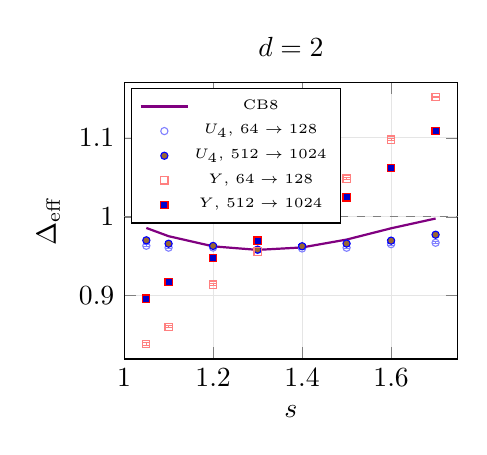
\begin{tikzpicture}
\begin{axis}[width=0.48\textwidth,height=0.42\textwidth,xlabel={$s$},ylabel={$\Delta_{\rm eff}$},title={$d=2$},xmin=1.0,xmax=1.75,ymin=0.82,ymax=1.17,
 legend style={font=\tiny,at={(0.02,0.98)},anchor=north west},grid=major,grid style={gray!20}]
\addplot[dashed,gray,forget plot] coordinates {(1.0,1) (1.75,1)};
\addplot[thick,violet] coordinates {(1.05,0.98584) (1.1,0.97543) (1.2,0.96257) (1.3,0.95810) (1.4,0.96118) (1.5,0.97114) (1.6,0.98542) (1.7,0.99780)};
\addlegendentry{CB8}
\addplot+[only marks,mark=o,mark size=1.3pt,blue!50,error bars/.cd,y dir=both,y explicit] coordinates {(1.05,0.9633) +- (0,0.0013) (1.1,0.9609) +- (0,0.0014) (1.2,0.9610) +- (0,0.0012) (1.3,0.9581) +- (0,0.0012) (1.4,0.9599) +- (0,0.0012) (1.5,0.9608) +- (0,0.0012) (1.6,0.9653) +- (0,0.0012) (1.7,0.9671) +- (0,0.0011)};
\addlegendentry{$U_4$, $64\rightarrow 128$}
\addplot+[only marks,mark=*,mark size=1.3pt,blue,error bars/.cd,y dir=both,y explicit] coordinates {(1.05,0.9702) +- (0,0.0025) (1.1,0.9659) +- (0,0.0023) (1.2,0.9631) +- (0,0.0022) (1.3,0.9584) +- (0,0.0020) (1.4,0.9627) +- (0,0.0020) (1.5,0.9661) +- (0,0.0018) (1.6,0.9698) +- (0,0.0018) (1.7,0.9773) +- (0,0.0017)};
\addlegendentry{$U_4$, $512\rightarrow 1024$}
\addplot+[only marks,mark=square,mark size=1.3pt,red!50,error bars/.cd,y dir=both,y explicit] coordinates {(1.05,0.8390) +- (0,0.0014) (1.1,0.8608) +- (0,0.0015) (1.2,0.9142) +- (0,0.0013) (1.3,0.9561) +- (0,0.0012) (1.4,1.0024) +- (0,0.0012) (1.5,1.0484) +- (0,0.0011) (1.6,1.0977) +- (0,0.0011) (1.7,1.1516) +- (0,0.0010)};
\addlegendentry{$Y$, $64\rightarrow 128$}
\addplot+[only marks,mark=square*,mark size=1.3pt,red,error bars/.cd,y dir=both,y explicit] coordinates {(1.05,0.8964) +- (0,0.0023) (1.1,0.9172) +- (0,0.0023) (1.2,0.9478) +- (0,0.0022) (1.3,0.9698) +- (0,0.0020) (1.4,0.9977) +- (0,0.0019) (1.5,1.0245) +- (0,0.0017) (1.6,1.0620) +- (0,0.0015) (1.7,1.1088) +- (0,0.0014)};
\addlegendentry{$Y$, $512\rightarrow 1024$}
\end{axis}
\end{tikzpicture}\hfill
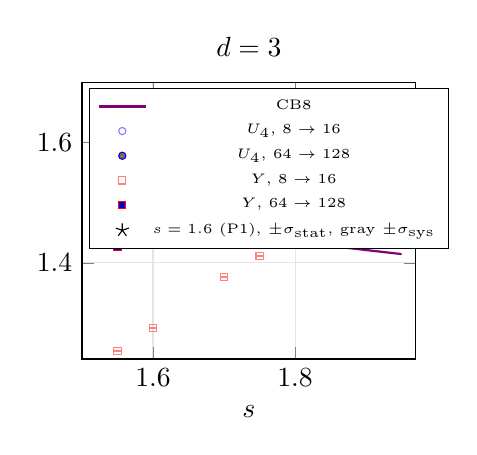
\begin{tikzpicture}
\begin{axis}[width=0.48\textwidth,height=0.42\textwidth,xlabel={$s$},title={$d=3$},xmin=1.5,xmax=1.97,ymin=1.24,ymax=1.70,
 legend style={font=\tiny,at={(0.02,0.98)},anchor=north west},grid=major,grid style={gray!20}]
\addplot[thick,violet] coordinates {(1.55,1.48488) (1.6,1.47214) (1.7,1.45154) (1.75,1.44299) (1.8,1.43524) (1.85,1.42807) (1.9,1.42123) (1.95,1.41449)};
\addlegendentry{CB8}
\addplot+[only marks,mark=o,mark size=1.3pt,blue!50,error bars/.cd,y dir=both,y explicit] coordinates {(1.55,1.4427) +- (0,0.0011) (1.6,1.4398) +- (0,0.0011) (1.7,1.4411) +- (0,0.0011) (1.75,1.4377) +- (0,0.0011) (1.8,1.4372) +- (0,0.0011) (1.85,1.4364) +- (0,0.0011) (1.9,1.4370) +- (0,0.0010) (1.95,1.4320) +- (0,0.0011)};
\addlegendentry{$U_4$, $8\rightarrow 16$}
\addplot+[only marks,mark=*,mark size=1.3pt,blue,error bars/.cd,y dir=both,y explicit] coordinates {(1.55,1.4729) +- (0,0.0030) (1.6,1.4715) +- (0,0.0031) (1.7,1.4650) +- (0,0.0029) (1.75,1.4615) +- (0,0.0027) (1.8,1.4515) +- (0,0.0027) (1.85,1.4569) +- (0,0.0027) (1.9,1.4511) +- (0,0.0026) (1.95,1.4493) +- (0,0.0028)};
\addlegendentry{$U_4$, $64\rightarrow 128$}
\addplot+[only marks,mark=square,mark size=1.3pt,red!50,error bars/.cd,y dir=both,y explicit] coordinates {(1.55,1.2535) +- (0,0.0012) (1.6,1.2914) +- (0,0.0013) (1.7,1.3761) +- (0,0.0012) (1.75,1.4115) +- (0,0.0012) (1.8,1.4513) +- (0,0.0012) (1.85,1.4929) +- (0,0.0012) (1.9,1.5325) +- (0,0.0012) (1.95,1.5694) +- (0,0.0011)};
\addlegendentry{$Y$, $8\rightarrow 16$}
\addplot+[only marks,mark=square*,mark size=1.3pt,red,error bars/.cd,y dir=both,y explicit] coordinates {(1.55,1.4269) +- (0,0.0030) (1.6,1.4628) +- (0,0.0030) (1.7,1.5263) +- (0,0.0029) (1.75,1.5596) +- (0,0.0027) (1.8,1.5818) +- (0,0.0027) (1.85,1.6221) +- (0,0.0027) (1.9,1.6488) +- (0,0.0025) (1.95,1.6790) +- (0,0.0027)};
\addlegendentry{$Y$, $64\rightarrow 128$}
\addplot+[only marks,mark=none,draw=none,forget plot,error bars/.cd,y dir=both,y explicit,error bar style={line width=3pt,gray!45},error mark=none] coordinates {(1.6,1.47314) +- (0,0.00230)};
\addplot+[only marks,mark=star,mark size=2.5pt,black,error bars/.cd,y dir=both,y explicit] coordinates {(1.6,1.47314) +- (0,0.00118)};
\addlegendentry{$s=1.6$ (P1), $\pm\sigma_{\rm stat}$, gray $\pm\sigma_{\rm sys}$}
\end{axis}
\end{tikzpicture}
\caption{Effective dimensions at the smallest and the largest doubling pair, with the resummed $\varepsilon$ expansion (CB8). Left, $d=2$
(dashed: $\De=1$ at both ends of the window). Right, $d=3$; the star is the value at $s=1.6$ that passed the protocol under P1, with $\sstat$
(bar) and $\ssys$ (gray band) shown separately. At the largest pair the $Y$ points (red) and the $U_4$ points (blue) agree in the middle of the
window and differ near its ends. In $d=2$ the difference shrinks as $L$ doubles at every coupling; in $d=3$ it shrinks at $s=1.55$ and 1.6 and
grows at $s\ge1.7$.}\label{fig:23}
\end{figure}

\clearpage
% =====================================================================================================================
\section{Synthesis}\label{sec:synthesis}
\begin{enumerate}[1.]
\item In $d=1$ nine couplings pass the protocol, with $\sstat=(2$--$5.5)\times10^{-4}$; they differ from the resummed $\varepsilon$ expansion
 by $-0.0024$ to $+0.0032$. $\ssys$ is a sensitivity scale. The audit supports the values at 0.1, 0.1375 and 0.1727335, which are stable under
 stronger size cuts. It flags 0.025 (a model outside the family) and 0.175 and 0.225 (stronger size cuts). The labels at 0.1625 and 0.1727335
 are platform-sensitive; two quoted fits have $P_{\chi^2}\approx5\times10^{-5}$; for $\Ds\ge0.0875$ the
 global fits lie above the crossing extrapolations by a common $0.0010(3)$.
\item In $d=2,3$ the finite-size data are precise ($\sigma(\Deff^{U_4})\approx0.0017$--$0.0031$ at the largest pair) and the bottleneck is the
 extrapolation: four doubling pairs over a factor 16 in $L$ do not determine the correction sector, especially near the ends of the window,
 where the expected correction exponents are below the grid floor. More statistics at the same sizes would sharpen, not resolve, this.
\item One 3D value passes, at $s=1.6$, under the post hoc amendment P1, and agrees with the expansion.
\item With a fitted correction exponent, a bootstrap at fixed exponent under-covers badly for single series; re-profiling the exponent in every
 draw restores coverage, conditionally on the extrapolation model.
\item The published equilibrium Monte Carlo values agree with ours within about two of their errors (in $d=1$ computed with $\sstat$, not
 $\ssys$); quantitative statements should use $\sstat$ and $\ssys$ separately.
\end{enumerate}

% =====================================================================================================================
\section{Open issues and next steps}\label{sec:open}
\begin{enumerate}[1.]
\item \textbf{1D uncertainties:} a pre-declared broader model family (a $U$ background, two correction powers, stronger size cuts), asymmetric
 model ranges, a converged $\omega'$ minimization and a ladder rule that does not stop on a flagged lower-degree fit, followed by a full rerun
 of the selection. Priority couplings: 0.025, 0.175, 0.225. A label-stability study (seeds, ladder rules, grid steps) belongs here.
\item \textbf{1D goodness of fit:} a $p$-value gate or a scale factor instead of $\chi^2/{\rm dof}\le1.5$.
\item \textbf{Near the Gaussian end} in all dimensions: a crossover form $D(L)=1+CL^{-\varepsilon}$ with free amplitudes, or $\omega$ fixed at its
 perturbative value, instead of a grid with floor 0.2.
\item \textbf{Near the short-range end} ($d=2,3$): the crossover flow of section~\ref{sec:model} as a model for the $Y$--$U_4$ split; measuring
 the effective $\eta$ at the crossings would test it.
\item \textbf{Larger lattices}, only where they answer a question: 2D $L=2048$ at $s=1.2$ and $1.5$; 3D $L=256$ at $s=1.9$ (about
 $1.5\times10^4$ core-hours), to tell an ordinary correction power from the slow short-range crossover by whether the $Y$--$U_4$ split grows or
 shrinks at $128\to256$.
\item \textbf{Critical inverse temperatures:} extrapolate $\beta_\times(L)$ with errors from the existing bootstrap draws.
\item \textbf{Uninspected code:} the last fixes to the P1 implementation and to the 1D tooling that records which campaigns make up each
 coupling (the registry).
\end{enumerate}

% =====================================================================================================================
\section{Reproduction}\label{sec:repro}
\sloppy
\subsection{The released folder}
This note is released with the code and the records in the \path{MC/} folder of the public repository (code under the MIT license, everything else under CC~BY~4.0, except the delivered 2D/3D
engine, which keeps its own MIT license); paths
below are relative to \path{MC/}. \code{README.md} states what is computed and its status; \code{REPRODUCE.md} gives the steps in order
(environment, tests, replay, smoke run, production, merge, checks) and the decisions that a reproduction must not take on its own.
\begin{description}[leftmargin=1.2em,font=\ttfamily]
\item[code/1d/] 1D engines (\path{src/}, \path{src_1d/}), campaign tools, analysis (\code{analyze.py}, \code{merge\_summaries.py},
 \code{equilibration.py}, \code{union\_check.py}), fitting (\code{select\_model\_v3.py}, \code{select\_model.py}, \code{fit\_fss.py},
 \code{quotients.py}), the 20-point report (\code{scan\_v3\_report.py}) and tests.
\item[code/2d3d\_engine/] the $d=2,3$ sampler and its analysis (\code{pack\_histograms.py}, \code{multihist.py},
 \code{precision\_analysis.py}) and tests.
\item[code/2d/, code/3d/] the evaluators (frozen rule and P1) and planners.
\item[code/reanalysis\_p1/] \code{calibrate\_p1.py} and the tests of amendment P1.
\item[code/package\_tools/] workspace assembly, the output comparison and the generator of this note's tables.
\item[protocols/] the analysis protocols, the amendment and their history (\code{PROTOCOL\_HISTORY.md}; appendix~\ref{app:hashes}).
\item[data/] the merged production records (\code{DATA.md}): 1D per-coupling selected fit runs, snapshot manifests, completion evidence and
 registries; 2D/3D analysis records at three block sizes, campaign manifests, histogram indices and the pinned production evaluations;
 reference values (\path{data/reference/}).
\item[results/] expected outputs: the P1 evaluations, the P1 calibration (an input of the P1 evaluation), the 1D tables and figures, and the
 cited diagnostics (cross-platform refits, the robust-ladder study with its modified fitter, the cross-check study).
\item[slurm/] submission templates with placeholders for account, partition and paths.
\end{description}
The evaluators bind themselves, the calibration script and the protocols by SHA-256 and locate their inputs relative to the layout they ran in;
the make targets therefore assemble that layout in a hidden \path{.work/} directory (code copied byte for byte, data linked), so every check
passes without any edit. The production records are released byte-identical, with one exception: 25 records (from the $d=1$ couplings
$\Ds=0.225$ and $0.2375$, and the P1 calibration) named a personal machine and were scrubbed after the results; only host labels, a home
directory and file names were replaced, and the hashes inside them re-pinned. \code{RE-PINNED.json} lists their original and published
SHA-256; the comparison maps one to the other. The other records name the cluster paths, user and compute nodes on which they were written.

\subsection{How to run}
Requirements: Python with NumPy and SciPy (production: Python 3.8.5, NumPy 1.19.2, SciPy 1.5.2 for the 1D fits; Python 3.8.8, NumPy 1.20.1
for the P1 calibration and evaluations; also tested with 3.12.3, 1.26.4, 1.11.4), pytest, matplotlib, a C++17 compiler and GNU make for the
engines, and pdflatex for this note.
\begin{longtable}{@{}>{\raggedright\arraybackslash}p{2.6cm}>{\raggedright\arraybackslash}p{6.5cm}>{\raggedright\arraybackslash}p{6.5cm}@{}}\toprule
target & runs & reproduces \\\midrule\endhead
\code{test} & builds the engines; 1D protocol tests; the tests of amendment P1 & the verification claims of section~\ref{sec:p1} \\
\code{replay} & everything below that needs only the records in git, then the comparison with \path{results/} & every table and figure of
 this note except those needing \code{fetch-data} \\
\code{smoke} & engine validation: a tiny 1D campaign with bitwise resume; exact enumeration and bitwise restart in $d=2,3$ & that the samplers are
 exact on small systems \\
\code{eval-fixed}, \code{eval-p1} & the 2D/3D evaluators under the frozen rule and under P1 & tables~\ref{tab:2ddec}, \ref{tab:3ddec};
 appendix~\ref{app:series} \\
\code{calibration} & \code{calibrate\_p1.py} (1\,780 tasks, $\approx7$~min on 16 cores) & appendix~\ref{app:calib} and the coverage numbers \\
\code{scan1d}, \code{tables1d} & \code{scan\_v3\_report.py}, \code{make\_tables\_and\_figure.py} & tables~\ref{tab:1dfinal}, \ref{tab:1dpairs},
 appendix~\ref{app:pre} \\
\code{refit1d DS=\dots} & \code{select\_model\_v3.py} on the released snapshot of one coupling (6--156~s on 20 cores); needs \code{fetch-data} &
 the fits, crossing series and label of that coupling; section~\ref{sec:1drefit} \\
\code{note-tables} & \code{make\_note\_tables.py --check} & every generated line of this note \\
\code{fetch-data}, \code{build}, \code{note} & downloads the data not in git; the engines; this note (three passes) & -- \\\bottomrule
\end{longtable}
\addtocounter{table}{-1}

\subsection{Verified reproduction}
On 7 October 2026 the folder, in its layout before the public release, was assembled afresh on the workstation and every target was run
through Slurm. The engines built and all tests passed. The 2D/3D evaluations reproduced the pinned production evaluations in all per-point
fields (maximum relative difference $3\times10^{-11}$), and so did the P1 evaluations and the calibration regenerated from scratch
($2\times10^{-11}$). The 1D cross-check study, the 20-point 1D table and the 1D report tables were reproduced, and the 1D fitting stage
reproduced 18 of 20 labels and all values (section~\ref{sec:1drefit}). The comparison reports those two labels as known to be platform-sensitive.

On 13 October 2026 the folder in its public layout was exported afresh and tested through Slurm on two platforms: a personal desktop (Python 3.12.3,
NumPy 1.26.4, SciPy 1.11.4) and an Expanse debug node (Python 3.8.8, NumPy 1.20.1, SciPy 1.6.2, GCC 10.2.0). On both, the engines build, all tests
pass (3.1 and 7.5~min), and \code{make replay} (14 and 43~s) reports 9 checks PASS, none FAIL and one NOT RUN, the regenerated calibration, which
needs \code{make calibration}; \code{note-tables} finds all 355 generated lines in this note. The cited 1D refits need \code{fetch-data} and
were not part of this test.

\subsection{What is not in git}
\code{make fetch-data} downloads two archives from the project's Zenodo data record, \href{https://doi.org/10.5281/zenodo.23466766}{doi:10.5281/zenodo.23466766}, and checks their SHA-256 (\code{data/HOSTED.json}).
\code{refit1d} needs the first: the 1D block archives of the selected snapshots (1.43~GB) and their merged summaries (25~MB). The second
holds the per-degree fits of the selected runs (140~MB), for inspection; no target needs them. Regenerating the records from scratch needs
the raw data: the 1D trajectories (0.655~TB) and the 2D/3D trees of chains, packed histograms and analyses (257.5 and 237.2~GiB). They are
not hosted; they are available from the author on request. The records were produced from
these by \code{analyze.py} and \code{merge\_summaries.py} ($d=1$) and by \code{pack\_histograms.py} and \code{precision\_analysis.py} ($d=2,3$).

% =====================================================================================================================
\appendix
\section{\texorpdfstring{$d=1$ frozen window parameters}{d=1 frozen window parameters}}\label{app:pre}
The window parameters $(\beta_c^{\rm pre},\De^{\rm pre})$ were frozen per coupling from earlier fits of the stage A/B data
(section~\ref{sec:rules}); $h'$ is the N2 temperature half-width.
\begin{table}[htbp]\centering\small
\caption{Frozen $(\beta_c^{\rm pre},\De^{\rm pre})$ per coupling and N2 half-widths $h'$ (units $10^{-4}$) at $N=2^{16}$ and $2^{19}$.}
\begin{tabular}{@{}lllllll@{}}\toprule
$\Ds$ & $s$ & $\beta_c^{\rm pre}$ & $\De^{\rm pre}$ & $h'(2^{16})$ & $h'(2^{19})$ & N2 \\\midrule
0.0125 & 0.975 & 0.596534 & 0.7910 & 14.67 & 9.50 & no \\
0.025 & 0.95 & 0.558588 & 0.7179 & 10.83 & 6.02 & no \\
0.0375 & 0.925 & 0.527150 & 0.6575 & 8.42 & 4.13 & no \\
0.05 & 0.9 & 0.499660 & 0.6234 & 7.31 & 3.34 & no \\
0.0625 & 0.875 & 0.474858 & 0.5898 & 6.35 & 2.71 & yes \\
0.075 & 0.85 & 0.452099 & 0.5674 & 5.79 & 2.35 & no \\
0.0875 & 0.825 & 0.430939 & 0.5462 & 5.30 & 2.06 & no \\
0.1 & 0.8 & 0.411095 & 0.5292 & 4.94 & 1.86 & yes \\
0.1125 & 0.775 & 0.392343 & 0.5191 & 4.74 & 1.74 & yes \\
0.125 & 0.75 & 0.374529 & 0.5074 & 4.51 & 1.62 & yes \\
0.1375 & 0.725 & 0.357528 & 0.4991 & 4.36 & 1.54 & yes \\
0.15 & 0.7 & 0.341247 & 0.4930 & 4.25 & 1.48 & yes \\
0.1625 & 0.675 & 0.325592 & 0.4863 & 4.13 & 1.42 & yes \\
0.1727335 & 0.654533 & 0.313200 & 0.4845 & 4.10 & 1.40 & yes \\
0.175 & 0.65 & 0.310504 & 0.4843 & 4.10 & 1.40 & yes \\
0.1875 & 0.625 & 0.295925 & 0.4814 & 4.05 & 1.38 & yes \\
0.2 & 0.6 & 0.281805 & 0.4808 & 4.04 & 1.37 & yes \\
0.2125 & 0.575 & 0.268101 & 0.4775 & 3.98 & 1.34 & yes \\
0.225 & 0.55 & 0.254785 & 0.4802 & 4.03 & 1.37 & yes \\
0.2375 & 0.525 & 0.241813 & 0.4809 & 4.04 & 1.37 & yes \\
\bottomrule\end{tabular}
\end{table}

\section{\texorpdfstring{$d=2,3$ extrapolation series}{d=2,3 extrapolation series}}\label{app:series}
For every coupling and series: $\De$ of the extrapolation, $\omega'$ and its $\Delta\chi^2\le1$ interval, $\chi^2$/dof, $\sigma$ with $\omega'$
fixed and profiled per draw (P1), eligibility.
{\scriptsize
\begin{longtable}{@{}llllllll@{}}
\caption{$d=2$ series (P1 evaluation; central values identical to the frozen evaluation).}\\\toprule
$s$ & series & $\De$ & $\omega'$ [interval] & $\chi^2$/dof & $\sigma$ fixed & $\sigma$ profiled & eligible \\\midrule\endfirsthead
\multicolumn{8}{@{}l}{\emph{$d=2$ series, continued}}\\\toprule
$s$ & series & $\De$ & $\omega'$ [interval] & $\chi^2$/dof & $\sigma$ fixed & $\sigma$ profiled & eligible \\\midrule\endhead
1.05 & U4 & 0.9750 & 0.56 [0.20, 2.00] & 0.51/1 & 0.0020 & 0.0083 & no: $\omega^\prime$ edge \\
 & U6 & 0.9719 & 0.84 [0.20, 2.00] & 0.29/1 & 0.0014 & 0.0080 & no: $\omega^\prime$ edge \\
 & U8 & 0.9700 & 0.96 [0.20, 2.00] & 0.14/1 & 0.0011 & 0.0087 & no: $\omega^\prime$ edge \\
 & Y & 0.9208 & 0.60 [0.43, 0.76] & 0.44/1 & 0.0018 & 0.0177 & yes \\
 & U4+Y & 0.9840 & 0.26 [0.26, 0.27] & 8.33/4 & 0.0037 & 0.0042 & no: $\chi^2$ \\
1.1 & U4 & 0.9670 & 1.17 [0.20, 2.00] & 0.11/1 & 0.0011 & 0.0060 & no: $\omega^\prime$ edge \\
 & U6 & 0.9663 & 1.33 [0.20, 2.00] & 0.10/1 & 0.0010 & 0.0060 & no: $\omega^\prime$ edge \\
 & U8 & 0.9651 & 1.41 [0.39, 2.00] & 0.03/1 & 0.0009 & 0.0067 & no: $\omega^\prime$ edge \\
 & Y & 0.9285 & 0.80 [0.61, 1.00] & 1.10/1 & 0.0015 & 0.0101 & yes \\
 & U4+Y & 0.9720 & 0.35 [0.35, 0.36] & 15.28/4 & 0.0028 & 0.0031 & no: $\chi^2$ \\
1.2 & U4 & 0.9654 & 0.20 [0.20, 2.00] & 3.57/1 & 0.0045 & 0.0043 & no: $\chi^2$ \\
 & U6 & 0.9657 & 0.20 [0.20, 1.44] & 3.66/1 & 0.0044 & 0.0042 & no: $\chi^2$ \\
 & U8 & 0.9686 & 0.20 [0.20, 0.78] & 2.73/1 & 0.0040 & 0.0044 & no: $\chi^2$ \\
 & Y & 0.9806 & 0.34 [0.20, 0.60] & 0.00/1 & 0.0027 & 0.0237 & no: $\omega^\prime$ edge \\
 & U4+Y & 0.9620 & 0.55 [0.53, 0.57] & 5.85/4 & 0.0016 & 0.0018 & yes \\
1.3 & U4 & 0.9595 & 2.00 [0.20, 2.00] & 0.49/1 & 0.0007 & 0.0030 & no: $\omega^\prime$ edge \\
 & U6 & 0.9595 & 2.00 [0.20, 2.00] & 0.56/1 & 0.0007 & 0.0029 & no: $\omega^\prime$ edge \\
 & U8 & 0.9595 & 2.00 [0.20, 2.00] & 0.70/1 & 0.0007 & 0.0036 & no: $\omega^\prime$ edge \\
 & Y & 0.9714 & 2.00 [1.58, 2.00] & 0.72/1 & 0.0007 & 0.0012 & no: $\omega^\prime$ edge \\
 & U4+Y & 0.9832 & 0.20 [0.20, 0.20] & 201.09/4 & 0.0042 & 0.0042 & no: $\chi^2$ \\
1.4 & U4 & 0.9624 & 0.20 [0.20, 2.00] & 2.38/1 & 0.0042 & 0.0035 & no: $\chi^2$ \\
 & U6 & 0.9643 & 0.20 [0.20, 2.00] & 2.30/1 & 0.0041 & 0.0038 & no: $\chi^2$ \\
 & U8 & 0.9689 & 0.20 [0.20, 1.32] & 1.83/1 & 0.0039 & 0.0044 & no: $\omega^\prime$ edge \\
 & Y & 0.9868 & 0.20 [0.20, 0.76] & 1.85/1 & 0.0042 & 0.0051 & no: $\omega^\prime$ edge \\
 & U4+Y & 0.9730 & 0.20 [0.20, 0.20] & 93.97/4 & 0.0040 & 0.0040 & no: $\chi^2$ \\
1.5 & U4 & 0.9759 & 0.20 [0.20, 0.98] & 0.48/1 & 0.0042 & 0.0055 & no: $\omega^\prime$ edge \\
 & U6 & 0.9777 & 0.20 [0.20, 0.92] & 0.46/1 & 0.0041 & 0.0056 & no: $\omega^\prime$ edge \\
 & U8 & 0.9819 & 0.20 [0.20, 0.91] & 0.29/1 & 0.0039 & 0.0064 & no: $\omega^\prime$ edge \\
 & Y & 0.9810 & 0.20 [0.20, 0.27] & 3.15/1 & 0.0038 & 0.0055 & no: $\chi^2$ \\
 & U4+Y & 0.9792 & 0.20 [0.20, 0.20] & 18.48/4 & 0.0038 & 0.0038 & no: $\chi^2$ \\
1.6 & U4 & 0.9799 & 0.20 [0.20, 0.97] & 1.09/1 & 0.0041 & 0.0053 & no: $\omega^\prime$ edge \\
 & U6 & 0.9822 & 0.20 [0.20, 1.10] & 0.59/1 & 0.0041 & 0.0057 & no: $\omega^\prime$ edge \\
 & U8 & 0.9839 & 0.25 [0.20, 1.47] & 0.18/1 & 0.0031 & 0.0063 & no: $\omega^\prime$ edge \\
 & Y & 0.9919 & 0.20 [0.20, 0.23] & 6.34/1 & 0.0035 & 0.0050 & no: $\chi^2$ \\
 & U4+Y & 0.9915 & 0.20 [0.20, 0.20] & 56.29/4 & 0.0035 & 0.0035 & no: $\chi^2$ \\
1.7 & U4 & 0.9984 & 0.20 [0.20, 0.66] & 0.51/1 & 0.0039 & 0.0087 & no: $\omega^\prime$ edge \\
 & U6 & 1.0012 & 0.20 [0.20, 0.75] & 0.50/1 & 0.0038 & 0.0093 & no: $\omega^\prime$ edge \\
 & U8 & 0.9935 & 0.36 [0.20, 0.97] & 0.57/1 & 0.0021 & 0.0097 & no: $\omega^\prime$ edge \\
 & Y & 1.0311 & 0.20 [0.20, 0.23] & 5.82/1 & 0.0034 & 0.0038 & no: $\chi^2$ \\
 & U4+Y & 1.0260 & 0.20 [0.20, 0.20] & 225.45/4 & 0.0034 & 0.0034 & no: $\chi^2$ \\
\bottomrule
\end{longtable}
\begin{longtable}{@{}llllllll@{}}
\caption{$d=3$ series (P1 evaluation).}\\\toprule
$s$ & series & $\De$ & $\omega'$ [interval] & $\chi^2$/dof & $\sigma$ fixed & $\sigma$ profiled & eligible \\\midrule\endfirsthead
\multicolumn{8}{@{}l}{\emph{$d=3$ series, continued}}\\\toprule
$s$ & series & $\De$ & $\omega'$ [interval] & $\chi^2$/dof & $\sigma$ fixed & $\sigma$ profiled & eligible \\\midrule\endhead
1.55 & U4 & 1.4812 & 0.75 [0.44, 1.11] & 0.00/1 & 0.0017 & 0.0163 & yes \\
 & U6 & 1.4809 & 0.79 [0.51, 1.10] & 0.02/1 & 0.0016 & 0.0139 & yes \\
 & U8 & 1.4790 & 0.92 [0.71, 1.15] & 0.02/1 & 0.0013 & 0.0075 & yes \\
 & Y & 1.4486 & 1.05 [0.99, 1.11] & 0.02/1 & 0.0014 & 0.0058 & yes \\
 & U4+Y & 1.4789 & 0.78 [0.78, 0.79] & 44.76/4 & 0.0015 & 0.0017 & no: $\chi^2$ \\
1.6 & U4 & 1.4726 & 1.29 [0.93, 1.74] & 0.28/1 & 0.0011 & 0.0072 & yes \\
 & U6 & 1.4720 & 1.35 [1.02, 1.75] & 0.29/1 & 0.0011 & 0.0062 & yes \\
 & U8 & 1.4709 & 1.39 [1.14, 1.67] & 0.37/1 & 0.0010 & 0.0040 & yes \\
 & Y & 1.4750 & 1.21 [1.14, 1.28] & 1.51/1 & 0.0013 & 0.0048 & yes \\
 & U4+Y & 1.4731 & 1.24 [1.23, 1.25] & 2.38/4 & 0.0011 & 0.0012 & yes \\
1.7 & U4 & 1.4737 & 0.66 [0.28, 1.09] & 0.07/1 & 0.0017 & 0.0168 & yes \\
 & U6 & 1.4724 & 0.74 [0.40, 1.14] & 0.03/1 & 0.0015 & 0.0157 & yes \\
 & U8 & 1.4700 & 0.92 [0.67, 1.20] & 0.02/1 & 0.0012 & 0.0082 & yes \\
 & Y & 1.5414 & 1.16 [1.08, 1.24] & 0.02/1 & 0.0012 & 0.0050 & yes \\
 & U4+Y & 1.4862 & 2.00 [2.00, 2.00] & 7052.05/4 & 0.0008 & 0.0008 & no: $\chi^2$ \\
1.75 & U4 & 1.4587 & 1.69 [1.03, 2.00] & 2.89/1 & 0.0009 & 0.0062 & no: $\chi^2$ \\
 & U6 & 1.4583 & 1.75 [1.17, 2.00] & 3.47/1 & 0.0009 & 0.0047 & no: $\chi^2$ \\
 & U8 & 1.4581 & 1.65 [1.28, 2.00] & 3.84/1 & 0.0009 & 0.0033 & no: $\chi^2$ \\
 & Y & 1.5654 & 1.35 [1.27, 1.44] & 4.12/1 & 0.0011 & 0.0041 & no: $\chi^2$ \\
 & U4+Y & 1.6546 & 0.20 [0.20, 0.20] & 10550.66/4 & 0.0050 & 0.0050 & no: $\chi^2$ \\
1.8 & U4 & 1.4553 & 2.00 [1.53, 2.00] & 2.02/1 & 0.0009 & 0.0016 & no: $\chi^2$ \\
 & U6 & 1.4551 & 2.00 [1.59, 2.00] & 2.37/1 & 0.0009 & 0.0015 & no: $\chi^2$ \\
 & U8 & 1.4542 & 2.00 [1.62, 2.00] & 2.76/1 & 0.0008 & 0.0016 & no: $\chi^2$ \\
 & Y & 1.5918 & 1.55 [1.46, 1.64] & 5.46/1 & 0.0010 & 0.0030 & no: $\chi^2$ \\
 & U4+Y & 1.6897 & 0.20 [0.20, 0.20] & 11986.04/4 & 0.0050 & 0.0050 & no: $\chi^2$ \\
1.85 & U4 & 1.4583 & 1.20 [0.71, 1.85] & 0.04/1 & 0.0010 & 0.0075 & yes \\
 & U6 & 1.4589 & 1.17 [0.76, 1.68] & 0.01/1 & 0.0010 & 0.0062 & yes \\
 & U8 & 1.4592 & 1.19 [0.92, 1.50] & 0.00/1 & 0.0009 & 0.0045 & yes \\
 & Y & 1.6306 & 1.39 [1.30, 1.48] & 0.20/1 & 0.0010 & 0.0034 & yes \\
 & U4+Y & 1.6685 & 0.20 [0.20, 0.20] & 14600.83/4 & 0.0045 & 0.0045 & no: $\chi^2$ \\
1.9 & U4 & 1.4545 & 1.15 [0.63, 1.87] & 0.89/1 & 0.0011 & 0.0072 & yes \\
 & U6 & 1.4544 & 1.23 [0.78, 1.81] & 0.83/1 & 0.0011 & 0.0057 & yes \\
 & U8 & 1.4546 & 1.29 [1.00, 1.64] & 0.83/1 & 0.0009 & 0.0034 & yes \\
 & Y & 1.6563 & 1.63 [1.53, 1.74] & 2.91/1 & 0.0009 & 0.0026 & no: $\chi^2$ \\
 & U4+Y & 1.6896 & 0.20 [0.20, 0.20] & 13764.62/4 & 0.0046 & 0.0046 & no: $\chi^2$ \\
1.95 & U4 & 1.4500 & 2.00 [1.56, 2.00] & 0.49/1 & 0.0008 & 0.0014 & no: $\omega^\prime$ edge \\
 & U6 & 1.4498 & 2.00 [1.61, 2.00] & 0.39/1 & 0.0008 & 0.0013 & no: $\omega^\prime$ edge \\
 & U8 & 1.4490 & 2.00 [1.64, 2.00] & 0.05/1 & 0.0007 & 0.0014 & no: $\omega^\prime$ edge \\
 & Y & 1.6827 & 2.00 [1.88, 2.00] & 0.70/1 & 0.0008 & 0.0014 & no: $\omega^\prime$ edge \\
 & U4+Y & 1.6808 & 0.20 [0.20, 0.20] & 19130.26/4 & 0.0048 & 0.0048 & no: $\chi^2$ \\
\bottomrule
\end{longtable}}

\section{P1 calibration strata}\label{app:calib}
Each cell: eligible synthetic fits: profiled $1\sigma$/$2\sigma$ coverage (fixed-$\omega'$ $1\sigma$ coverage), status (P pass, F fail, nc not
calibrated, i.e.\ fewer than 200 eligible fits). Last column: synthetic sets with $U_4$ and $Y$ both eligible: false-failure rate of the profiled
cross-check (fixed), status.
\begin{sidewaystable}\centering\footnotesize\setlength{\tabcolsep}{4pt}
\caption{Calibration strata of amendment P1 (top $d=2$, bottom $d=3$).}\label{tab:calib}
\begin{tabular}{@{}lllllll@{}}\toprule
$d=2$, $s$ & $U_4$ & $U_6$ & $U_8$ & $Y$ & U4+Y & cross-check \\\midrule
1.05 & 0 nc & 0 nc & 19: 1.00/1.00 (0.16) nc & 1493: 0.83/0.95 (0.12) P & 1812: 0.68/0.95 (0.59) P & 0 nc \\
1.1 & 0 nc & 1: 1.00/1.00 (0.00) nc & 8: 1.00/1.00 (0.00) nc & 1672: 0.83/0.95 (0.15) P & 1799: 0.69/0.96 (0.63) P & 0 nc \\
1.2 & 0 nc & 0 nc & 0 nc & 490: 0.33/0.82 (0.00) F & 1805: 0.67/0.95 (0.62) P & 0 nc \\
1.3 & 0 nc & 0 nc & 0 nc & 196: 1.00/1.00 (0.01) nc & 194: 0.10/0.44 (0.01) nc & 0 nc \\
1.4 & 0 nc & 0 nc & 0 nc & 0 nc & 15: 0.87/1.00 (0.87) nc & 0 nc \\
1.5 & 1: 0.00/1.00 (0.00) nc & 0 nc & 3: 0.00/1.00 (0.00) nc & 234: 0.00/0.02 (0.00) F & 0 nc & 0 nc \\
1.6 & 0 nc & 0 nc & 2: 1.00/1.00 (0.00) nc & 222: 0.00/0.03 (0.00) F & 0 nc & 0 nc \\
1.7 & 62: 0.00/0.13 (0.00) nc & 69: 0.00/0.10 (0.00) nc & 144: 0.40/1.00 (0.00) nc & 214: 0.00/0.04 (0.00) F & 0 nc & 0 nc \\
\bottomrule\end{tabular}\\[12pt]
\begin{tabular}{@{}lllllll@{}}\toprule
$d=3$, $s$ & $U_4$ & $U_6$ & $U_8$ & $Y$ & U4+Y & cross-check \\\midrule
1.55 & 1225: 0.86/0.98 (0.19) P & 1396: 0.87/0.97 (0.17) P & 1666: 0.83/0.96 (0.17) P & 1663: 0.69/0.95 (0.20) P & 1771: 0.68/0.95 (0.63) P & 1062: 0.007 (0.69) P \\
1.6 & 1122: 0.99/1.00 (0.31) P & 1165: 0.98/1.00 (0.31) P & 1378: 0.88/1.00 (0.29) P & 1668: 0.69/0.95 (0.21) P & 1786: 0.70/0.95 (0.67) P & 1076: 0.007 (0.61) P \\
1.7 & 825: 0.92/1.00 (0.20) P & 1107: 0.90/1.00 (0.19) P & 1603: 0.89/0.97 (0.16) P & 1671: 0.69/0.96 (0.18) P & 218: 0.29/0.89 (0.06) F & 108: 0.000 (0.43) nc \\
1.75 & 428: 1.00/1.00 (0.01) P & 420: 0.98/1.00 (0.02) P & 684: 0.81/1.00 (0.15) P & 1710: 0.69/0.95 (0.23) P & 47: 0.00/0.09 (0.00) nc & 108: 0.000 (0.76) nc \\
1.8 & 228: 0.99/1.00 (0.00) P & 246: 0.95/1.00 (0.01) P & 229: 0.41/1.00 (0.02) F & 1645: 0.70/0.96 (0.26) P & 1: 0.00/0.00 (0.00) nc & 79: 0.000 (0.87) nc \\
1.85 & 717: 1.00/1.00 (0.32) P & 996: 1.00/1.00 (0.27) P & 1483: 0.93/1.00 (0.23) P & 1695: 0.70/0.96 (0.22) P & 0 nc & 93: 0.108 (1.00) nc \\
1.9 & 531: 1.00/1.00 (0.38) P & 764: 1.00/1.00 (0.32) P & 1289: 0.98/1.00 (0.32) P & 1663: 0.71/0.97 (0.29) P & 0 nc & 92: 0.326 (1.00) nc \\
1.95 & 216: 1.00/1.00 (0.00) P & 237: 0.99/1.00 (0.01) P & 254: 0.47/1.00 (0.00) F & 182: 0.15/0.84 (0.01) nc & 0 nc & 39: 0.641 (1.00) nc \\
\bottomrule\end{tabular}
\end{sidewaystable}

\section{Protocol identities and history}\label{app:hashes}
SHA-256 prefixes of the files whose identity matters (full hashes in \path{protocols/} and in the records):
FIT\_MODEL\_V3 rev.\ 14 \code{f05b835b}; FIT\_MODEL\_2D rev.\ 5 \code{4d2efc63}; FIT\_MODEL\_3D rev.\ 5 (approved) \code{b4ccf436} and rev.\ 7
(production) \code{682858f0}; amendment P1 rev.\ 4 \code{2a18c0ae}; frozen evaluators \code{evaluate\_2d.py} rev.\ 5 \code{0fe221e8} and
\code{evaluate\_3d.py} rev.\ 1 \code{6bd35d7a}; P1 evaluators rev.\ 6 \code{3c3e35fc} and rev.\ 2 \code{d635c917}; \code{calibrate\_p1.py}
\code{d94b59f2}; calibration \code{CALIBRATION.json} \code{897142c1}; production evaluations \code{fbfc0ef9} (2D) and \code{ae9cf237} (3D); P1
evaluations \code{f9272978} (2D) and \code{b3fd6364} (3D). Records that named a personal machine were scrubbed after the results and
re-pinned; \code{RE-PINNED.json} lists the original and published hashes (for example \code{CALIBRATION.json}: original \code{897142c1},
published \code{1afae79a}, which differ only in a host label). The prefixes above are the original ones.

The file \code{FIT\_MODEL\_3D.md.sha256} records the hash at approval (revision 5), while the evaluators pin revision 7. The approved revision 5,
revision 6 and the difference to revision 7 are released (\path{protocols/FIT_MODEL_3D_rev5_approved.md}, \dots); the two differ only in
the preflight condition and the gate records described in section~\ref{sec:rules}. \code{FIT\_MODEL\_2D.md} has no approval hash because it
was never approved. The status lines inside the protocol files (for example ``UNREVIEWED'') predate their reviews; \code{PROTOCOL\_HISTORY.md}
gives the review status of each revision.

\section{\texorpdfstring{The pre-campaign $\varepsilon$-expansion reference}{The pre-campaign epsilon-expansion reference}}\label{app:eps}
Before the campaign, six-loop reference values were computed and frozen with the records
(\path{data/1d/reference/published_and_epsilon_reference.csv}); they played no role in any selection. ``GFF only'' (generalized free field, i.e.\ the Gaussian end) is the ordinary
Borel--Pad\'e [4/2] of the six-loop series about the Gaussian end; ``endpoint assisted'' is the Borel--Pad\'e [3/3] of the remainder $R$ in
$\De=1-\sqrt{1-e}+(1-e)/8+(1-e)^{3/2}R(e)$, $e=\varepsilon$, which builds in the $s\to1$ endpoint behavior. They used an older value of the six-loop coefficient of the $d=1$ series, $C_6(1)=14331.8\pm0.5$; the final value, 14331.687, is given in the
accompanying article~\cite{Zheng:2026ai}. They are superseded by the eight-loop values of section~\ref{sec:theory1d}. The same
file contains columns from an exploratory pre-campaign analysis (\code{new\_MC\_conditional\_fit} and related), which are also superseded.
\begin{table}[htbp]\centering\small
\caption{$d=1$: the frozen six-loop reference values against the Monte Carlo result.}\label{tab:eps}
\begin{tabular}{@{}lllll@{}}\toprule
$\Ds$ & $\varepsilon=1-4\Ds$ & six-loop, GFF only & six-loop, endpoint assisted & MC (this work) \\\midrule
0.025 & 0.900 & 0.5703 & 0.7109 & 0.71115(49)(959) \\
0.05 & 0.800 & 0.5459 & 0.6182 & 0.61987(55)(220) \\
0.0625 & 0.750 & 0.5351 & 0.5871 & 0.59003(35)(150) \\
0.1 & 0.600 & 0.5085 & 0.5262 & 0.53248(20)(242) \\
0.15 & 0.400 & 0.4871 & 0.4897 & 0.49325(41)(306) \\
0.1727335 & 0.309 & 0.4829 & 0.4836 & 0.48368(52)(78) \\
0.2 & 0.200 & 0.4828 & 0.4829 & largest pair \\
\bottomrule\end{tabular}
\end{table}

\section{Glossary}
\begin{description}[leftmargin=1.2em]
\item[$\Ds$, $\De$] dimensions of the spin and of the leading $\mathbb Z_2$-even scalar; $1/\nu=d-\De$.
\item[$\Deff^Q$] finite-size effective dimension from a doubling pair at the $U_4$ crossing, eq.~\eqref{eq:Deff}.
\item[$\sstat$, $\ssys$, $\sigma_D$] bootstrap error of the quoted value; half-range over the model family (a sensitivity scale, not a standard
 deviation); error of a paired difference.
\item[$p$, $\ktau$] polynomial degree of the scaling function; order of the thermal field ($d=1$ fits).
\item[$P_{\chi^2}$] $\chi^2$ probability of a fit.
\item[coupling] one value of $s$ (or $\Ds$) of the simulation grid; inverse temperatures are $\beta$.
\item[window, variant, configuration] in $d=1$: the range $|x|\le x_{\max}$ of the scaling variable kept in a fit; the form of the correction
 terms (\code{leading}, \code{second}, \code{background}, \code{log}); one choice of window, variant, $N_{\min}$ and $\ktau$
 (section~\ref{sec:v3}).
\item[gate] a pass/fail condition on a fit or series.
\item[quotable, eligible] a $d=1$ fit that passes its gates; a $d=2,3$ extrapolation series that passes its gates.
\item[series] $\Deff^Q(L)$ over the doubling pairs for one $Q$ ($d=2,3$) or one crossing window and degree rule ($d=1$), extrapolated to
 $L\to\infty$.
\item[U4+Y] joint extrapolation of $U_4$ and $Y$ with common $\De$ and $\omega'$.
\item[x-check] cross-check (table~\ref{tab:labels}).
\item[{[$\sigma$]}] label suffix: $\sigma(\Deff^{U_4})$ of the largest pair above the target 0.003.
\item[frozen] fixed before the data in question were analyzed (a protocol, the $d=1$ window parameters); ``the frozen rule'' is the
 $d=2,3$ protocol before amendment P1.
\item[fixed-$\omega'$ / profiled rule] bootstrap at the central $\omega'$ (the frozen rule) / $\omega'$ re-profiled in every draw (amendment P1).
\item[preflight] short runs at the production sizes, before a production, that check rates, autocorrelation times and crossing brackets.
\item[stage 0, A, B; N0, N2, N3] 1D campaigns (table~\ref{tab:campaigns}); N3, an extension to $N=2^{20}$, was not run.
\item[N1] the first evaluation of all 20 $d=1$ couplings with protocol v3 (section~\ref{sec:rules}).
\item[snapshot] an immutable, hashed set of merged summaries from which one fit run is made.
\item[CB8] the eight-loop $\varepsilon$ expansion of the accompanying article, resummed by conformal Borel resummation with the short-range end
 imposed.
\end{description}

\begin{thebibliography}{99}\small
\bibitem{Zheng:2026ai} Z.~Zheng, \emph{The long-range Ising CFT: perturbative and nonperturbative approaches}, in preparation (2026).
\bibitem{Chang:2024whx} C.-H. Chang, V.~Dommes, R.~S. Erramilli, A.~Homrich, P.~Kravchuk, A.~Liu, M.~S. Mitchell, D.~Poland and
 D.~Simmons-Duffin, \emph{Bootstrapping the 3d Ising stress tensor}, JHEP \textbf{03} (2025) 136, arXiv:2411.15300.
\bibitem{LeGuillou:1979ixc} J.~C. Le~Guillou and J.~Zinn-Justin, \emph{Critical exponents from field theory}, Phys.\ Rev.\ B \textbf{21}, 3976 (1980).
\bibitem{Fisher:1972zz} M.~E. Fisher, S.-k. Ma and B.~G. Nickel, \emph{Critical exponents for long-range interactions}, Phys.\ Rev.\ Lett.\ \textbf{29}, 917 (1972).
\bibitem{Sak:1973oqx} J.~Sak, \emph{Recursion relations and fixed points for ferromagnets with long-range interactions}, Phys.\ Rev.\ B \textbf{8}, 281 (1973).
\bibitem{Paulos:2015jfa} M.~F. Paulos, S.~Rychkov, B.~C. van Rees and B.~Zan, \emph{Conformal invariance in the long-range Ising model}, Nucl.\ Phys.\ B \textbf{902}, 246 (2016), arXiv:1509.00008.
\bibitem{Behan:2017dwr} C.~Behan, L.~Rastelli, S.~Rychkov and B.~Zan, \emph{Long-range critical exponents near the short-range crossover}, Phys.\ Rev.\ Lett.\ \textbf{118}, 241601 (2017), arXiv:1703.03430.
\bibitem{Behan:2017emf} C.~Behan, L.~Rastelli, S.~Rychkov and B.~Zan, \emph{A scaling theory for the long-range to short-range crossover and an infrared duality}, J.\ Phys.\ A \textbf{50}, 354002 (2017), arXiv:1703.05325.
\bibitem{Kosterlitz:1976zz} J.~M. Kosterlitz, \emph{Phase transitions in long-range ferromagnetic chains}, Phys.\ Rev.\ Lett.\ \textbf{37}, 1577 (1976).
\bibitem{Cardy:1981xx} J.~L. Cardy, \emph{One-dimensional models with $1/r^2$ interactions}, J.\ Phys.\ A \textbf{14}, 1407 (1981).
\bibitem{Binder:1981sa} K.~Binder, \emph{Finite size scaling analysis of Ising model block distribution functions}, Z.\ Phys.\ B \textbf{43}, 119 (1981).
\bibitem{Ballesteros:1996bd} H.~G. Ballesteros, L.~A. Fern\'andez, V.~Mart\'{\i}n-Mayor and A.~Mu\~noz Sudupe, \emph{Finite size effects on measures of critical exponents in $d=3$ O($N$) models}, Phys.\ Lett.\ B \textbf{387}, 125 (1996), arXiv:cond-mat/9606203.
\bibitem{Swendsen:1987ce} R.~H. Swendsen and J.-S. Wang, \emph{Nonuniversal critical dynamics in Monte Carlo simulations}, Phys.\ Rev.\ Lett.\ \textbf{58}, 86 (1987).
\bibitem{Fukui:2009on} K.~Fukui and S.~Todo, \emph{Order-N cluster Monte Carlo method for spin systems with long-range interactions}, J.\ Comput.\ Phys.\ \textbf{228}, 2629 (2009), arXiv:0802.0272.
\bibitem{Horita:2017ul} T.~Horita, H.~Suwa and S.~Todo, \emph{Upper and lower critical decay exponents of Ising ferromagnets with long-range interaction}, Phys.\ Rev.\ E \textbf{95}, 012143 (2017), arXiv:1605.09496.
\bibitem{Luijten:1995mc} E.~Luijten and H.~W.~J. Bl\"ote, \emph{Monte Carlo method for spin models with long-range interactions}, Int.\ J.\ Mod.\ Phys.\ C \textbf{6}, 359 (1995).
\bibitem{Shirts:2008xx} M.~R. Shirts and J.~D. Chodera, \emph{Statistically optimal analysis of samples from multiple equilibrium states}, J.\ Chem.\ Phys.\ \textbf{129}, 124105 (2008).
\bibitem{Ferrenberg:1989ui} A.~M. Ferrenberg and R.~H. Swendsen, \emph{Optimized Monte Carlo data analysis}, Phys.\ Rev.\ Lett.\ \textbf{63}, 1195 (1989).
\bibitem{Uzelac:2001lc} K.~Uzelac, Z.~Glumac and A.~Ani\v{c}i\'c, \emph{Critical behavior of the long-range Ising chain from the largest-cluster probability distribution}, Phys.\ Rev.\ E \textbf{63}, 037101 (2001), arXiv:cond-mat/0011306.
\bibitem{Angelini:2014koy} M.~C. Angelini, G.~Parisi and F.~Ricci-Tersenghi, \emph{Relations between short-range and long-range Ising models}, Phys.\ Rev.\ E \textbf{89}, 062120 (2014), arXiv:1401.6805.
\bibitem{Luijten:1997th} E.~Luijten, \emph{Interaction range, universality and the upper critical dimension}, PhD thesis, Delft University of Technology (1997).
\bibitem{Luijten:1997cl} E.~Luijten and H.~W.~J. Bl\"ote, \emph{Classical critical behavior of spin models with long-range interactions}, Phys.\ Rev.\ B \textbf{56}, 8945 (1997), arXiv:cond-mat/9704016.
\bibitem{Tomita:2009mc} Y.~Tomita, \emph{Monte Carlo study of one-dimensional Ising models with long-range interactions}, J.\ Phys.\ Soc.\ Jpn.\ \textbf{78}, 014002 (2009).
\bibitem{Glumac:1989fr} Z.~Glumac and K.~Uzelac, \emph{Finite-range scaling study of the 1D long-range Ising model}, J.\ Phys.\ A \textbf{22}, 4439 (1989).
\bibitem{Picco:2012ak} M.~Picco, \emph{Critical behavior of the Ising model with long range interactions}, arXiv:1207.1018 (2012).
\bibitem{Xiao:2025sk} T.~Xiao, Z.~Liu, Z.~Fan and Y.~Deng, \emph{On Sak's criterion for statistical models with long-range interaction}, arXiv:2512.04805 (2025).
\bibitem{Behan:2018hfx} C.~Behan, \emph{Bootstrapping the long-range Ising model in three dimensions}, J.\ Phys.\ A \textbf{52}, 075401 (2019), arXiv:1810.07199.
\bibitem{Behan:2023ile} C.~Behan, E.~Lauria, M.~Nocchi and P.~van Vliet, \emph{Analytic and numerical bootstrap for the long-range Ising model}, JHEP \textbf{03} (2024) 136, arXiv:2311.02742.
\bibitem{Defenu:2014bea} N.~Defenu, A.~Trombettoni and A.~Codello, \emph{Fixed-point structure and effective fractional dimensionality for O($N$) models with long-range interactions}, Phys.\ Rev.\ E \textbf{92}, 052113 (2015), arXiv:1409.8322.
\end{thebibliography}
\end{document}
